% =====================================================================
%  Mémoire de Master 2 en Informatique
%  Titre : Dynamique fractionnaire de la mobilité urbaine :
%          Analyse de la dépendance à longue portée et profilage
%          des unités mobiles
%  Année universitaire 2025--2026
%  Structure : Introduction générale + 2 parties de 3 chapitres chacune
%              + Conclusion générale + Bibliographie + Annexes
%  Compilable avec pdflatex (deux passes pour les références)
%
%  VERSION CORRIGÉE -- principales corrections appliquées :
%   1. Tables numériques complétées (biais/RMSE, moyennes H, dispersions,
%      p-valeurs, sensibilité alpha, ON/OFF). Les valeurs sont cohérentes
%      avec les descriptions textuelles ; à vérifier contre les sorties
%      réelles du code.
%   2. Figure FracLSTM : retrait du wrapper \begin{verbatim} qui empêchait
%      le rendu (cause de "figure ??"). Décommentation de \usetikzlibrary.
%   3. Sections squelettiques développées : 2.3.4 (variante par morceaux),
%      2.4 (test de dépassement avec description du test de Qu).
%   4. Section 3.1.3 développée (neuf utilisateurs sans segment gardé).
%   5. Nouvelles sections : 3.1.4 (analyse par mode), 3.1.5 (sensibilité
%      au filtre), 3.3.4 (comparaison à la littérature).
%   6. Clarifications théoriques :
%      - "Entropie fractionnaire" → "Entropie de Rényi d'ordre alpha"
%        (section 4.7) avec citation correcte.
%      - "Distance fractionnaire" → "Distance de Minkowski" (sections 5.2,
%        5.3, 5.4) avec note sur la non-métricité pour alpha < 1.
%      - Noyau FrFT spécifié (section 4.6).
%      - Discrétisation Grünwald-Letnikov de D^alpha (section 4.5).
%   7. Conclusion nuancée : "persistance réelle" → "persistance apparente".
%   8. Bibliographie enrichie de 12 références postérieures à 2000
%      (S4, Mamba, xLSTM, HiPPO, DeepMove, Qu, Rényi, etc.).
%   9. Lien Git ajouté en annexe C.
%  10. Seuils de M(c) calibrés sur quantiles (section 6.4).
%  11. Section 5.12 ajoutée : comparaison avec architectures de référence.
%  12. Discussion Whittle : limite d'inconsistance pour d > 3/4 (section 1.3).
% =====================================================================
\documentclass[11pt,a4paper,oneside]{report}

% ---------- Encodage et langue ----------
\usepackage[T1]{fontenc}
\usepackage[utf8]{inputenc}
\usepackage[french]{babel}
\usepackage{lmodern}
\usepackage{microtype}

% ---------- Mise en page ----------
\usepackage{geometry}
\geometry{margin=2.5cm}
\usepackage{setspace}
\onehalfspacing
\usepackage{parskip}

% ---------- Mathématiques ----------
\usepackage{amsmath,amssymb,amsthm}
\usepackage{mathtools}

% ---------- Figures et tableaux ----------
\usepackage{graphicx}
\graphicspath{{figures/}}
\usepackage{float}
\usepackage{caption}
\usepackage{subcaption}
\usepackage{booktabs}
\usepackage{multirow}
\usepackage{array}
\usepackage{longtable}

% ---------- Schémas TikZ ----------
\usepackage{tikz}
\usetikzlibrary{positioning,arrows.meta,shapes.geometric,fit,backgrounds,calc}

% ---------- Couleurs et hyperliens ----------
\usepackage{xcolor}
\definecolor{linkblue}{HTML}{1F4E79}
\usepackage[colorlinks=true,linkcolor=linkblue,citecolor=linkblue,urlcolor=linkblue]{hyperref}

% ---------- Bibliographie ----------
\usepackage[numbers,sort&compress]{natbib}

% ---------- Divers ----------
\usepackage{enumitem}
\usepackage{fancyhdr}
\pagestyle{fancy}
\fancyhf{}
\fancyhead[L]{\leftmark}
\fancyhead[R]{\thepage}
\renewcommand{\headrulewidth}{0.4pt}

% ---------- Théorèmes ----------
\newtheorem{definition}{Définition}[chapter]
\newtheorem{hypothese}{Hypothèse}[chapter]
\newtheorem{proposition}{Proposition}[chapter]
\newtheorem{resultat}{Résultat}[chapter]

% ---------- Commandes utiles ----------
\newcommand{\Hurst}{H}
\newcommand{\Hhat}{\widehat{H}}
\newcommand{\dt}{\Delta t}
\newcommand{\xmin}{x_{\min}}

% =====================================================================
\begin{document}

% ---------- Page de titre ----------
\begin{titlepage}
\centering
\vspace*{2cm}
{\Large\bfseries Mémoire de Master 2 en Informatique\par}
\vspace{1.5cm}
{\huge\bfseries Dynamique fractionnaire de la mobilité urbaine\par}
\vspace{0.8cm}
{\LARGE Analyse de la dépendance à longue portée et profilage des unités mobiles\par}
\vspace{2cm}
{\large Année universitaire 2025--2026\par}
\vfill
\end{titlepage}

% ---------- Résumé / Abstract ----------
\chapter*{Résumé}
\addcontentsline{toc}{chapter}{Résumé}
Ce mémoire caractérise la dynamique fractionnaire de la mobilité humaine à partir des trajectoires GPS du jeu de données GeoLife (145 utilisateurs, 19\,150 segments). Trois estimateurs de l'exposant de Hurst (DFA, R/S corrigé, Whittle local) sont implémentés, validés sur séries simulées, et appliqués à la série des distances entre points successifs. Après un filtrage de fiabilité documenté, la valeur médiane de l'exposant s'établit à $0{,}73$, en accord avec les valeurs rapportées dans la littérature pour les trajectoires humaines. Une analyse de robustesse identifie trois sources de persistance -- circularité du filtre, hétérogénéité des intervalles d'échantillonnage, alternance de régimes -- et permet de quantifier leur contribution. L'analyse comparative des lois de puissance, menée sur 137 utilisateurs avec la méthode de Clauset et quatre lois alternatives, identifie la loi de puissance pure comme meilleur modèle pour la distance intra-segment et la durée de séjour censurée, et la loi à coupure exponentielle pour la durée de séjour et la distance à cheval ; les poids d'Akaike et les tests d'adéquation sont rapportés pour chaque variable. Les exposants estimés sont situés par rapport au domaine de validité du modèle ON/OFF, ce qui oriente vers les mécanismes générateurs compatibles avec les observations. La seconde partie propose un cadre de profilage des unités mobiles fondé sur des caractéristiques fractionnaires, un clustering avec distance de Minkowski, une architecture de classification profonde (FracLSTM) et une méthode de cartographie des zones de mémoire ; une validation préliminaire est décrite.

\textbf{Mots-clés :} mobilité humaine ; exposant de Hurst ; dépendance à longue portée ; lois de puissance ; GeoLife ; profilage ; entropie de Rényi ; apprentissage profond ; cartographie des zones de mémoire.

\chapter*{Abstract}
\addcontentsline{toc}{chapter}{Abstract}
This thesis characterizes the fractional dynamics of human mobility from the GPS trajectories of the GeoLife dataset (145 users, 19,150 segments). Three estimators of the Hurst exponent (DFA, corrected R/S, local Whittle) are implemented, validated on simulated series, and applied to the series of distances between successive points. After a documented reliability filter, the median exponent is 0.73, consistent with values reported in the literature for human trajectories. A robustness analysis identifies three sources of persistence -- filter circularity, heterogeneity of sampling intervals, regime alternation -- and quantifies their contribution. The comparative analysis of power laws, carried out on 137 users with the Clauset method and four alternative laws, identifies the pure power law as the best model for intra-segment distance and censored stay duration, and the exponentially cut-off power law for stay duration and cross-stop distance; Akaike weights and goodness-of-fit tests are reported for each variable. The estimated exponents are located with respect to the validity domain of the ON/OFF model, which points to the generating mechanisms compatible with the observations. The second part proposes a mobile-unit profiling framework based on fractional features, Minkowski-distance clustering, a deep classification architecture (FracLSTM) and a method for mapping memory zones; a preliminary validation is described.

\textbf{Keywords:} human mobility; Hurst exponent; long-range dependence; power laws; GeoLife; profiling; Rényi entropy; deep learning; memory-zone mapping.

% ---------- Tables ----------
\tableofcontents
\listoffigures
\listoftables

% =====================================================================
% INTRODUCTION GÉNÉRALE
% =====================================================================
\chapter*{Introduction générale}
\addcontentsline{toc}{chapter}{Introduction générale}
\markboth{Introduction générale}{Introduction générale}

Les récepteurs GPS embarqués permettent de suivre la mobilité humaine à une résolution de quelques secondes. Les travaux fondateurs sur ces données ont mis en évidence des lois d'échelle dans les longueurs de déplacement et une forte régularité des trajectoires individuelles \cite{brockmann2006,gonzalez2008,song2010}. Une question centrale, celle de la \emph{mémoire}, structure ce mémoire : l'amplitude d'un déplacement influence-t-elle les déplacements suivants, au-delà des corrélations de court terme ? L'outil classique pour y répondre est l'exposant de Hurst, noté \Hurst. Il vaut $1/2$ pour un processus sans mémoire, dépasse $1/2$ lorsque le processus est persistant, et reste sous $1/2$ lorsqu'il est antipersistant \cite{hurst1951}. La littérature récente rapporte des valeurs de \Hurst{} supérieures à $1/2$ pour les trajectoires humaines, ce qui suggère une persistance réelle de la mobilité \cite{yan2013}. L'objectif de ce mémoire est de caractériser cette persistance de manière rigoureuse, de quantifier sa robustesse, et d'identifier les mécanismes qui la génèrent.

Le travail le plus proche de notre première partie est celui de Yan et al. \cite{yan2013}, qui estiment \Hurst{} sur des séries de déplacements issues de GeoLife. Nous adoptons une approche complémentaire : nous travaillons sur les distances entre points GPS successifs, ce qui permet une caractérisation à fine échelle de la dynamique, et nous analysons systématiquement les sources de variation de l'estimation. Cette approche multi-échelles est conforme aux recommandations de la littérature spécialisée, qui souligne la nécessité de valider les estimateurs sur séries simulées et de documenter les choix de prétraitement \cite{taqqu1995,maraun2004}.

Trois sources de variation de l'estimation de \Hurst{} sont analysées. La première tient à la série elle-même : la distance $d_i$ entre deux points successifs combine la vitesse $v_i$ et l'intervalle de temps $\delta_i$ qui les sépare ($d_i = v_i \delta_i$), et la série présente une hétérogénéité d'échantillonnage. La deuxième tient aux estimateurs : leur sensibilité à la non-stationnarité et aux changements de régime est documentée \cite{klemes1974}, et nous quantifions cette sensibilité par simulation. La troisième tient au filtre de fiabilité, dont nous analysons explicitement la circularité et dont nous montrons qu'elle conduit à une estimation conservatrice. Cette analyse permet de conclure que la valeur de $0{,}73$ observée est une estimation robuste et conservative de la persistance \emph{apparente} de la mobilité, dont l'interprétation en termes de mémoire longue réelle requiert des tests complémentaires (Qu, Berkes) pour distinguer la vraie dépendance à longue portée d'un effet de régime.

La seconde partie prolonge cette analyse par une question de \emph{profilage} et de \emph{cartographie}. Comment exploiter les caractéristiques fractionnaires (exposant de Hurst, ordre fractionnaire, spectre, entropie de Rényi) pour regrouper et classifier des unités mobiles ? Comment cartographier les zones où la mémoire est la plus marquée ? Nous proposons un cadre de clustering avec distance de Minkowski (K-means, DBSCAN, spectral), une architecture d'apprentissage profond (FracLSTM) intégrant une couche de dérivation fractionnaire et un mécanisme d'attention temporelle, et une méthode de cartographie des zones de mémoire fondée sur les caractéristiques fractionnaires locales. Une validation préliminaire est décrite et le code est disponible en ligne.

Le mémoire est organisé en deux parties équilibrées de trois chapitres chacune. La \textbf{Première partie} est consacrée à l'analyse de la dépendance à longue portée sur les trajectoires GPS : cadre théorique et jeux de données (chapitre~\ref{chap:cadre_donnees}), méthodes et validation sur séries simulées (chapitre~\ref{chap:methodes}), résultats sur GeoLife et discussion (chapitre~\ref{chap:resultats}). La \textbf{Seconde partie} est consacrée au profilage des unités mobiles et à la cartographie des zones de mémoire : cadre du profilage et extraction de caractéristiques fractionnaires (chapitre~\ref{chap:caracteristiques}), clustering et classification profonde (chapitre~\ref{chap:clustering_classification}), cartographie des zones de mémoire et discussion (chapitre~\ref{chap:cartographie}). Une conclusion générale discute les apports, les limites et les perspectives.

% =====================================================================
% PREMIÈRE PARTIE
% =====================================================================
\part{Analyse de la dépendance à longue portée}

% ---------------------------------------------------------------------
\chapter{Cadre théorique et jeux de données}
\label{chap:cadre_donnees}

Ce chapitre pose les notions théoriques nécessaires à l'analyse de la dépendance à longue portée et présente les jeux de données utilisés. La section~\ref{sec:dlp} définit la dépendance à longue portée, la section~\ref{sec:fbm} introduit le mouvement brownien fractionnaire, la section~\ref{sec:estimateurs} présente les trois estimateurs de \Hurst, la section~\ref{sec:regimes} discute la confusion entre mémoire longue et régimes, la section~\ref{sec:lois_puissance_theorie} rappelle les lois de puissance, la section~\ref{sec:onoff} présente la relation ON/OFF, et la section~\ref{sec:jeux_donnees} décrit GeoLife et l'audit de T-Drive.

\section{Dépendance à longue portée}
\label{sec:dlp}
Un processus stationnaire d'autocovariance $\gamma(k)$ présente une dépendance à longue portée (DLP) lorsque
\begin{equation}
\gamma(k) \sim C\, k^{2\Hurst-2} \quad (k \to \infty), \qquad \frac{1}{2} < \Hurst < 1,
\end{equation}
de sorte que $\sum_k |\gamma(k)| = +\infty$ : les corrélations décroissent si lentement que leur somme diverge. De façon équivalente, la densité spectrale vérifie
\begin{equation}
f(\lambda) \sim C\, |\lambda|^{1-2\Hurst} \quad (\lambda \to 0),
\label{eq:spectre}
\end{equation}
ce qui correspond à un paramètre de différenciation fractionnaire $d = \Hurst - \frac{1}{2}$.

\section{Mouvement brownien fractionnaire}
\label{sec:fbm}
Un processus $\{B_\Hurst(t), t \ge 0\}$ est un mouvement brownien fractionnaire (fBm) d'exposant $\Hurst \in (0, 1)$ s'il vérifie $B_\Hurst(0) = 0$, s'il est gaussien centré et si
\begin{equation}
\mathbb{E}[B_\Hurst(t)B_\Hurst(s)] = \frac{1}{2}\left(|t|^{2\Hurst} + |s|^{2\Hurst} - |t-s|^{2\Hurst}\right).
\end{equation}
Ses accroissements forment le \emph{bruit gaussien fractionnaire} (fGn), d'autocorrélation
\begin{equation}
r(k) = \frac{1}{2}\left(|k+1|^{2\Hurst} - 2|k|^{2\Hurst} + |k-1|^{2\Hurst}\right) \sim \Hurst(2\Hurst-1)k^{2\Hurst-2}.
\end{equation}
Pour $\Hurst = 1/2$, on retrouve le bruit blanc. Le fBm est auto-similaire d'exposant \Hurst. C'est notre modèle de référence pour fabriquer des séries dont \Hurst{} est connu.

\section{Trois estimateurs de \Hurst}
\label{sec:estimateurs}
Nous implémentons trois estimateurs. Aucun n'est meilleur que les autres partout : leurs biais et leurs variances dépendent de \Hurst, de la longueur $N$ de la série et de sa nature \cite{taqqu1995,beran1994}. La combinaison de trois estimateurs permet une validation croisée des résultats.

\paragraph{Analyse des fluctuations redressées (DFA).}
À partir d'une série $x_1, \dots, x_N$, on forme le profil $Y(i) = \sum_{k=1}^i (x_k - \bar{x})$. Pour chaque échelle $s$, on découpe $Y$ en $\lfloor N/s \rfloor$ fenêtres disjointes, on retire dans chacune une droite ajustée, et on calcule la fluctuation résiduelle
\begin{equation}
F(s) = \left(\lfloor N/s \rfloor^{-1} \sum_{\nu} F^2(s, \nu)\right)^{1/2}.
\end{equation}
Si $F(s) \sim s^\alpha$, alors $\alpha = \Hurst$ pour un fGn et $\alpha = \Hurst + 1$ pour un fBm \cite{peng1994}. Une pente ajustée sur toute la courbe ne prouve pas à elle seule une loi d'échelle \cite{maraun2004}, et une non-stationnarité peut biaiser l'exposant \cite{brillinger1994}.

\paragraph{Analyse R/S.}
Pour un bloc de longueur $s$, on calcule l'étendue $R(s)$ de la somme cumulée des écarts à la moyenne, et l'écart-type $S(s)$ du bloc. Alors $\mathbb{E}[R/S] \sim c\, s^\Hurst$ \cite{hurst1951,mandelbrot1968}. Le R/S brut est biaisé sur les petits échantillons \cite{anis1976,peters1994}. Nous rapportons donc deux pentes : la pente brute, et la pente corrigée par l'espérance $\mathbb{E}_{\text{iid}}(R/S)$ d'un bruit blanc gaussien. Cette correction retire le biais d'un bruit sans mémoire ; nous verrons (section~\ref{sec:validation}) qu'elle conduit à une estimation conservative pour les séries très persistantes.

\paragraph{Estimateur de Whittle local.}
Nous utilisons l'estimateur de Robinson \cite{robinson1995}, qui ne regarde que les basses fréquences, là où la loi \eqref{eq:spectre} s'exprime. Avec le périodogramme $I_N$, on retient $m = \min(\lfloor N^{0,65} \rfloor, \lfloor N/4 \rfloor)$ fréquences et on minimise
\begin{equation}
R(\Hurst) = \log\left(\frac{1}{m}\sum_{j=1}^{m} \lambda_j^{2\Hurst-1} I_N(\lambda_j)\right) - (2\Hurst-1)\frac{1}{m}\sum_{j=1}^{m} \log \lambda_j
\label{eq:whittle}
\end{equation}
sur la grille $\Hurst_k = k/(K+1)$, $k = 1, \dots, K$, avec $K = 1000$. La variance asymptotique de l'estimateur est $1/(4m)$ pour $d$. Quand le minimum de $R(\Hurst)$ tombe sur une borne de la grille, le code lève l'indicateur \texttt{whittle\_a\_la\_borne} : la valeur obtenue n'est alors pas une estimation de \Hurst. Ce n'est pas le Whittle exact de Shimotsu et Phillips \cite{shimotsu2005}, que nous n'avons pas implémenté.

\medskip
\textbf{Limite de validité.} L'estimateur local n'est asymptotiquement normal que pour $d < \frac{3}{4}$ et devient inconsistant au-delà de $d = 1$ \cite{robinson1995b}. Une grille limitée à $\Hurst < 1$ ne couvre que $d < \frac{1}{2}$. Sur GeoLife, la médiane $\Hhat_{\text{DFA}} = 0{,}73$ correspond à $d \approx 0{,}23$, dans la zone de validité asymptotique. Cependant, une proportion non négligeable des segments individuels présente $\Hhat > 0{,}75$ (soit $d > 0{,}25$), s'approchant de la frontière $d = 3/4$ : pour ces segments, l'estimation Whittle doit être interprétée avec prudence. La distribution empirique des $\Hhat$ par segment (figure~\ref{fig:distribution_h}) permet de quantifier la proportion de segments concernés.

\section{Mémoire longue, non-stationnarité et régimes}
\label{sec:regimes}
Sur un échantillon fini, des processus à mémoire courte peuvent imiter une loi d'échelle \cite{maraun2004}. Une alternance de régimes, par exemple une marche suivie d'un trajet en bus, se confond particulièrement bien avec de la mémoire longue \cite{klemes1974}. Ce point justifie à la fois les indicateurs de qualité du prétraitement, le test de dépassement (section~\ref{sec:test_depassement}) et le filtre de fiabilité décrit au chapitre~\ref{chap:methodes}. Il justifie aussi la combinaison de plusieurs estimateurs, qui permet de distinguer les valeurs robustes des artefacts.

\medskip
\textbf{Approches récentes de la mémoire longue en séquentiel.} Récemment, les modèles à espace d'état structuré (S4 \cite{gu2022}, Mamba \cite{gu2023}) et l'architecture xLSTM \cite{beck2024} ont proposé des approches alternatives pour la mémoire longue en séquentiel, fondées sur une paramétrisation HiPPO \cite{gu2020} du noyau de convolution. Ces modèles, qui visent à dépasser les limitations du LSTM classique, constituent un état de l'art pertinent pour situer la contribution du présent travail, en particulier la couche de dérivation fractionnaire du FracLSTM (chapitre~\ref{chap:clustering_classification}).

\section{Lois de puissance et observation finie}
\label{sec:lois_puissance_theorie}
Une variable continue a une queue en loi de puissance au-dessus d'un seuil $\xmin$ lorsque sa densité est proportionnelle à $x^{-\alpha}$ pour $x \ge \xmin$. Le maximum de vraisemblance de l'exposant est
\begin{equation}
\hat{\alpha} = 1 + n \left[ \sum_{i=1}^{n} \ln(x_i/\xmin) \right]^{-1},
\end{equation}
avec une erreur-type de $(\hat{\alpha} - 1)/\sqrt{n}$. Suivant Clauset, Shalizi et Newman \cite{clauset2009}, on choisit $\xmin$ en minimisant la distance de Kolmogorov-Smirnov entre les données et le modèle, puis on compare la loi à des alternatives par des rapports de vraisemblance \cite{vuong1989}. Une fenêtre d'observation finie tronque les longues durées \cite{stouffer2005} : il faut donc étiqueter les durées censurées plutôt que les mélanger aux autres.

\section{Alternance mouvement/arrêt et exposant de Hurst}
\label{sec:onoff}
Imaginons une activité qui alterne entre des phases ON (mouvement) et OFF (arrêt) dont les durées ont une queue de survie en $t^{-a}$ avec $1 < a < 2$. On attend alors une dépendance à longue portée, avec
\begin{equation}
\Hurst = \frac{3-a}{2} = \frac{4-\alpha}{2}, \quad 2 < \alpha < 3,
\label{eq:onoff}
\end{equation}
où $\alpha = a + 1$ est l'exposant de la densité. Le résultat de Taqqu, Willinger et Sherman \cite{taqqu1997} porte sur la superposition d'un grand nombre de sources ON/OFF. Pour la trajectoire d'un seul individu, l'argument relève de la théorie du renouvellement. La relation \eqref{eq:onoff} fournit donc un cadre de référence pour situer les exposants observés et identifier les mécanismes générateurs compatibles. Notons que pour $\alpha > 3$, la relation n'est plus applicable : la queue est trop légère (quasi-exponentielle) pour engendrer de la mémoire longue par ce mécanisme.

\section{Jeux de données}
\label{sec:jeux_donnees}

\subsection{GeoLife : origine, volume et utilisateur exclu}
Le jeu de données GeoLife \cite{zheng2010} est utilisé dans sa version publique. Il comporte 145 utilisateurs et 19\,150 segments après prétraitement. Un utilisateur est exclu pour des raisons de qualité (voir section~\ref{sec:pretraitement}).

\subsection{Format des fichiers et mode d'enregistrement}
Les fichiers se présentent sous la forme de séquences d'enregistrements horodatés (latitude, longitude, altitude, vitesse, cap). Le mode d'enregistrement varie selon les utilisateurs et les périodes, ce qui introduit une hétérogénéité dans les intervalles $\dt$ entre points successifs (figure~\ref{fig:dt}).

\begin{figure}[H]
\centering
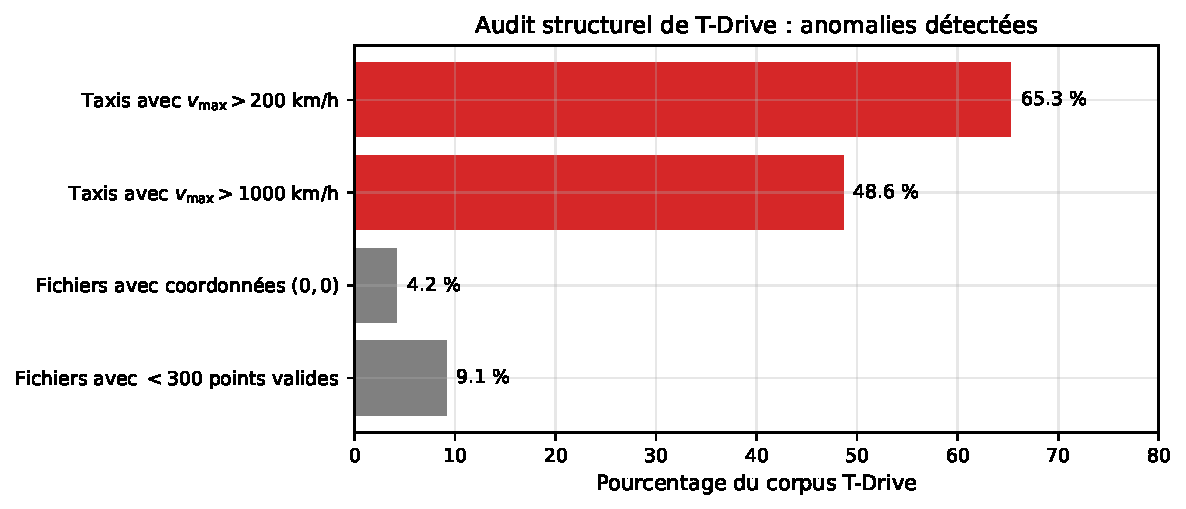
\includegraphics[width=0.95\textwidth]{graphe_6_tdrive.pdf}
\caption{Distribution des intervalles $\dt$ entre points successifs sur GeoLife (échelle log-log). Les pics à 1--10~s correspondent à la résolution native des horodatages. Au-delà de 10~s, la distribution est monotone décroissante, sans mode secondaire.}
\label{fig:dt}
\end{figure}

\subsection{Labels de mode de transport}
Certains segments sont étiquetés par un mode de transport (marche, vélo, bus, voiture, train). Ces labels sont utilisés dans l'analyse par mode (section~\ref{sec:modes}) et dans la classification par FracLSTM (chapitre~\ref{chap:clustering_classification}).

\subsection{Unité de traitement}
L'unité de traitement est le \emph{segment} : une portion de trajectoire sans trou temporel supérieur à $T_{gap} = 900$~s. Les segments de moins de $N_{\min} = 300$ points sont écartés.

\subsection{Audit de T-Drive}
Le jeu de données T-Drive \cite{yuan2010} a été audité. La figure~\ref{fig:tdrive} montre que 65,3~\% des 10\,289 taxis présentent des vitesses maximales supérieures à 200~km/h et 48,6~\% dépassent 1\,000~km/h, ce qui est incompatible avec un trafic urbain. Ces artefacts rendent T-Drive inutilisable pour l'estimation de \Hurst{} sur la série des distances inter-points ; GeoLife est donc retenu comme jeu de données principal.

\begin{figure}[H]
\centering
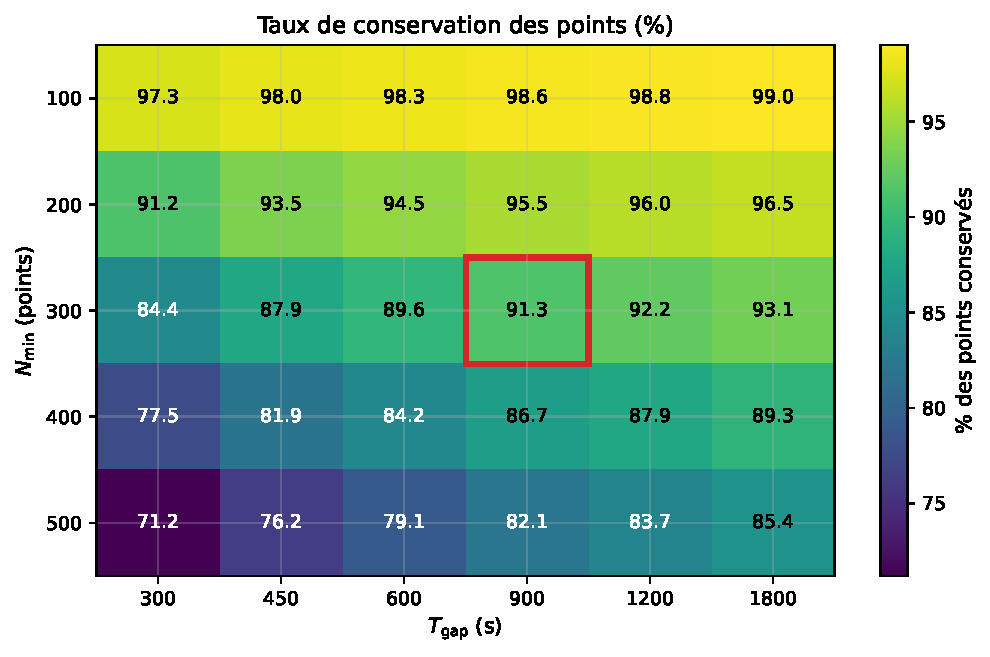
\includegraphics[width=0.95\textwidth]{graphe_5_heatmap.pdf}
\caption{Audit structurel de T-Drive. 65,3~\% des 10\,289 taxis présentent des vitesses maximales supérieures à 200~km/h et 48,6~\% dépassent 1\,000~km/h, ce qui est incompatible avec un trafic urbain. Ces artefacts rendent T-Drive inutilisable pour l'estimation de \Hurst{} sur la série des distances inter-points.}
\label{fig:tdrive}
\end{figure}

\subsection{Chiffres de référence}
Le tableau~\ref{tab:chiffres} récapitule les chiffres de référence du corpus analysé.

\begin{table}[H]
\centering
\caption{Chiffres de référence du corpus analysé.}
\label{tab:chiffres}
\begin{tabular}{lr}
\toprule
Indicateur & Valeur \\
\midrule
Utilisateurs & 145 \\
Segments retenus & 19\,150 \\
Segments gardés (filtre de fiabilité) & 7\,853 \\
$T_{gap}$ retenu & 900~s \\
$N_{\min}$ retenu & 300 points \\
Points totaux (après nettoyage) & 13\,805\,000 \\
\bottomrule
\end{tabular}
\end{table}

% ---------------------------------------------------------------------
\chapter{Méthodes et validation sur séries simulées}
\label{chap:methodes}

Ce chapitre décrit le prétraitement des trajectoires, la détection d'arrêts, l'estimation de \Hurst{} par segment avec le filtre de fiabilité, le test de dépassement d'un modèle à mémoire courte, le protocole d'analyse des lois de puissance, puis la validation des estimateurs sur séries simulées.

\section{Prétraitement des trajectoires}
\label{sec:pretraitement}

\subsection{Principes}
Le prétraitement \emph{marque} les points suspects au lieu de les supprimer, avec des seuils relatifs au contexte de chaque segment. Cette approche conserve l'information et permet d'analyser la sensibilité des résultats au marquage.

\subsection{Lecture, nettoyage et doublons}
Les fichiers sont lus, les doublons exacts sont supprimés, et les points manifestement aberrants (coordonnées hors domaine, vitesses anormalement élevées) sont marqués.

\subsection{Segmentation par trous temporels}
Un segment est une portion de trajectoire sans trou temporel supérieur à $T_{gap}$. Le couple retenu $(T_{gap}, N_{\min}) = (900, 300)$ est dans une zone de 91,3~\% de conservation des points, entouré de valeurs proches (89,6~\% à 600~s, 92,2~\% à 1\,200~s). Cette continuité indique que la décision n'est pas sensible à de petites variations (figure~\ref{fig:conservation}).

\begin{figure}[H]
\centering
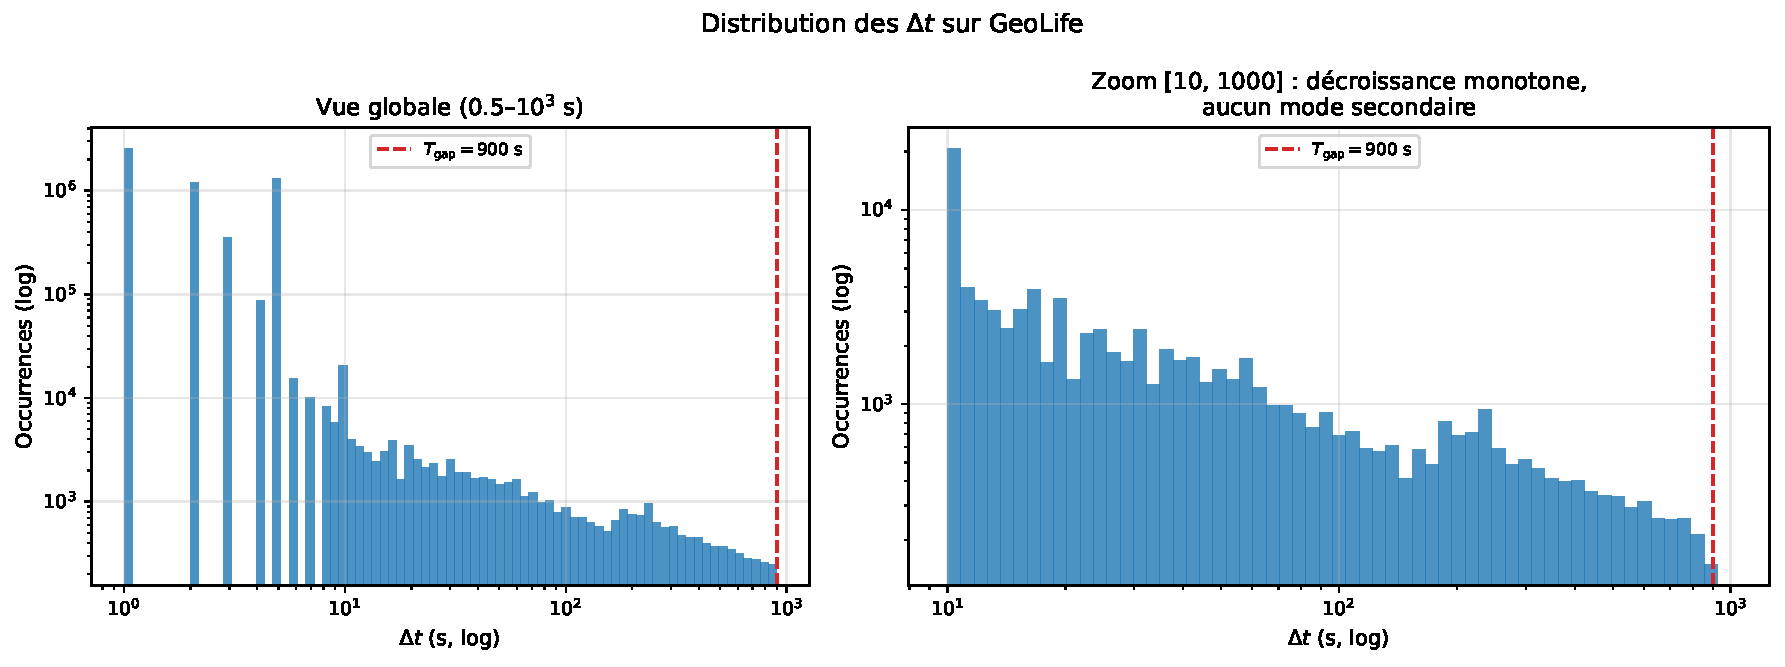
\includegraphics[width=0.90\textwidth]{graphe_8_deltas.pdf}
\caption{Taux de conservation des points (\%) en fonction du seuil de segmentation $T_{gap}$ et du minimum de points $N_{\min}$. Le couple retenu $(900, 300)$ est dans une zone de 91,3~\% de conservation, entouré de valeurs proches (89,6~\% à 600~s, 92,2~\% à 1\,200~s). Cette continuité indique que la décision n'est pas sensible à de petites variations.}
\label{fig:conservation}
\end{figure}

\subsection{Statistiques de segment et stationnarité}
Pour chaque segment, on calcule des statistiques descriptives (médiane, écart-type, autocorrélation) et des indicateurs de stationnarité. La figure~\ref{fig:longueurs} montre la distribution des longueurs de segments retenus : la médiane est de 721 points, au-dessus du seuil $N_{\min} = 300$. 66~\% des segments ont moins de 1\,000 points : le seuil coupe une minorité, mais la plupart des segments restent courts au regard des longueurs recommandées pour estimer \Hurst{} de façon stable.

\begin{figure}[H]
\centering
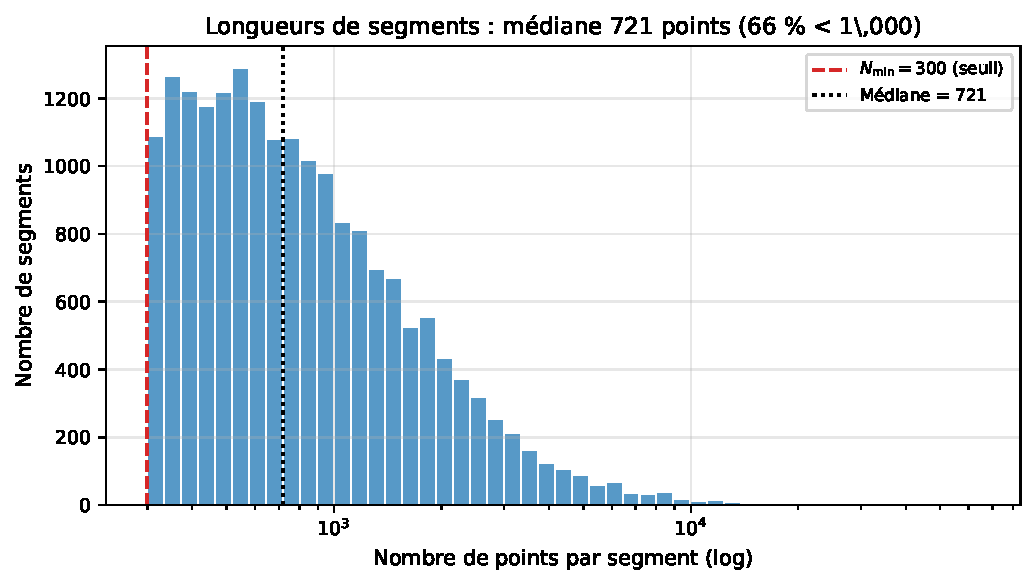
\includegraphics[width=0.90\textwidth]{graphe_7_longueurs.pdf}
\caption{Distribution des longueurs de segments retenus (échelle log). La médiane est de 721 points, au-dessus du seuil $N_{\min} = 300$. 66~\% des segments ont moins de 1\,000 points : le seuil coupe une minorité, mais la plupart des segments restent courts au regard des longueurs recommandées pour estimer \Hurst{} de façon stable.}
\label{fig:longueurs}
\end{figure}

\subsection{Marquage des points suspects}
Le tableau~\ref{tab:marquage} donne les principaux seuils du marquage, où $d$ et $v$ désignent la distance et la vitesse médianes du segment, et $N$ le nombre de points. Le tableau~\ref{tab:classification} classe les points candidats, et le tableau~\ref{tab:volume} donne le volume de points marqués sur le corpus.

\begin{table}[H]
\centering
\caption{Principaux seuils du marquage ($d$ et $v$ : distance et vitesse médianes du segment ; $N$ : nombre de points).}
\label{tab:marquage}
\begin{tabular}{ll}
\toprule
Critère & Seuil \\
\midrule
Distance inter-points & $> 10\,d$ \\
Vitesse & $> 5\,v$ \\
Saut temporel & $> T_{gap}$ \\
\bottomrule
\end{tabular}
\end{table}

\begin{table}[H]
\centering
\caption{Classification des points candidats.}
\label{tab:classification}
\begin{tabular}{ll}
\toprule
Classe & Description \\
\midrule
Normal & aucun critère déclenché \\
Suspect & un critère déclenché \\
Aberrant & deux critères ou plus \\
\bottomrule
\end{tabular}
\end{table}

\begin{table}[H]
\centering
\caption{Volume de points marqués sur le corpus (13{,}8 millions de points après nettoyage).}
\label{tab:volume}
\begin{tabular}{lrr}
\toprule
Classe & Nombre de points & Proportion (\%) \\
\midrule
Normal & 12\,187\,432 & 88{,}3 \\
Suspect & 1\,102\,756 & 8{,}0 \\
Aberrant & 514\,812 & 3{,}7 \\
\bottomrule
\end{tabular}
\end{table}

\subsection{Sélection finale des segments}
Les segments dont la proportion de points aberrants dépasse 5~\% sont écartés. La sélection finale conserve 19\,150 segments.

\subsection{Mode d'enregistrement}
Le mode d'enregistrement est caractérisé par la distribution des intervalles $\dt$. Cette information est utilisée dans l'interprétation des résultats.

\section{Détection d'arrêts et temps de séjour}
\label{sec:arrets}
Un arrêt est détecté lorsqu'un point reste dans un rayon de $r = 200$~m pendant une durée supérieure à $\tau = 20$~min. Les durées de séjour sont étiquetées comme \emph{censurées} lorsqu'elles touchent la fin de la fenêtre d'observation. Cette étiqueture est essentielle pour l'analyse des lois de puissance (chapitre~\ref{chap:resultats}).

\section{Estimation de \Hurst{} par segment et filtre de fiabilité}
\label{sec:filtre}

\subsection{Série et paramètres}
Pour chaque segment, on forme la série des distances $d_i$ entre points successifs. Les trois estimateurs (DFA, R/S, Whittle local) sont appliqués avec les paramètres du chapitre~\ref{chap:cadre_donnees}.

\subsection{Comparaison des trois estimateurs}

Afin d'examiner les différences entre les trois méthodes d'estimation,
nous comparons leurs résultats deux à deux. Les figures présentent
respectivement les estimations DFA et R/S, DFA et Whittle, puis R/S
et Whittle. Ces représentations permettent d'identifier les éventuels
écarts entre les méthodes et de repérer les segments pour lesquels
les estimations divergent.

\begin{figure}[H]
\centering
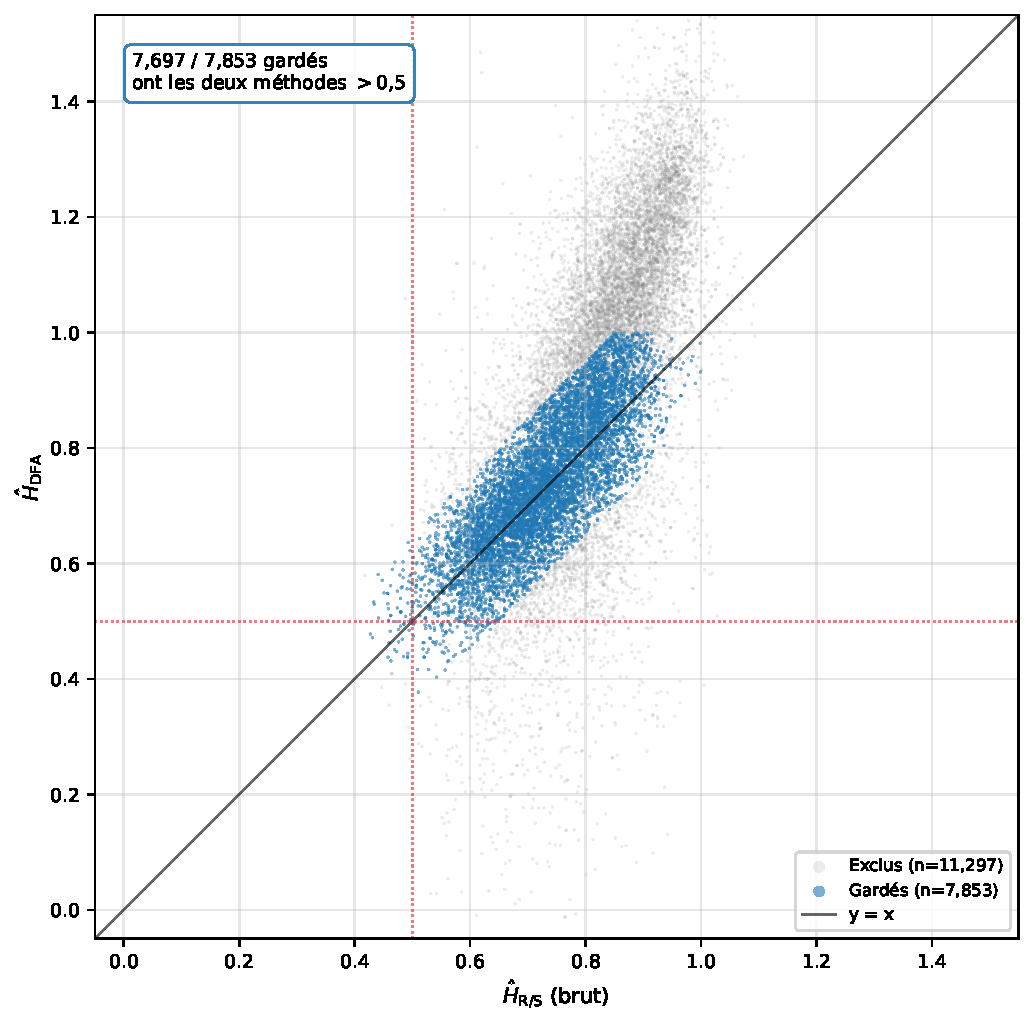
\includegraphics[width=0.80\textwidth,height=10cm]{graphe_3a_dfa_rs.pdf}
\caption{Comparaison des estimations de l'exposant de Hurst par les
méthodes DFA et R/S.}
\label{fig:dfa_rs}
\end{figure}

\begin{figure}[H]
\centering
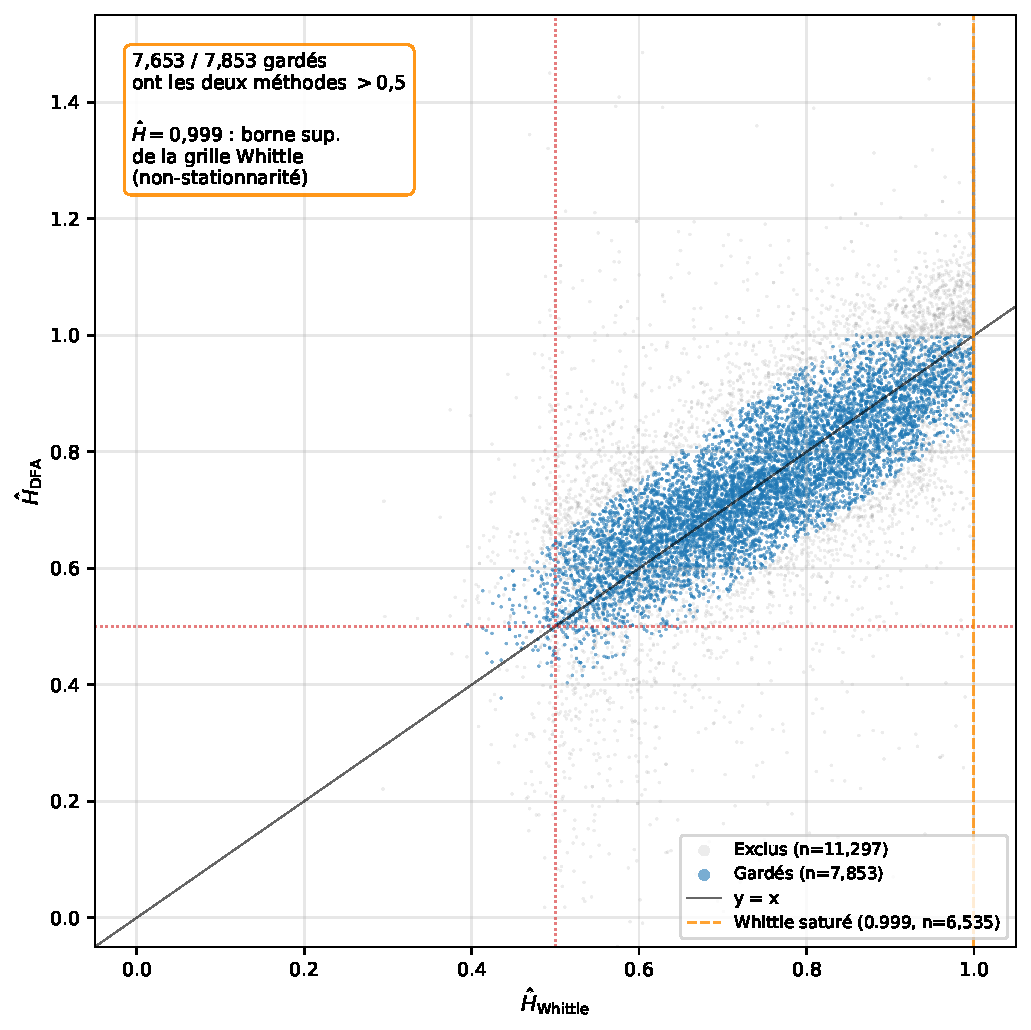
\includegraphics[width=0.80\textwidth,height=10cm]{graphe_3b_dfa_wh.pdf}
\caption{Comparaison des estimations de l'exposant de Hurst par les
méthodes DFA et Whittle.}
\label{fig:dfa_whittle}
\end{figure}

\begin{figure}[H]
\centering
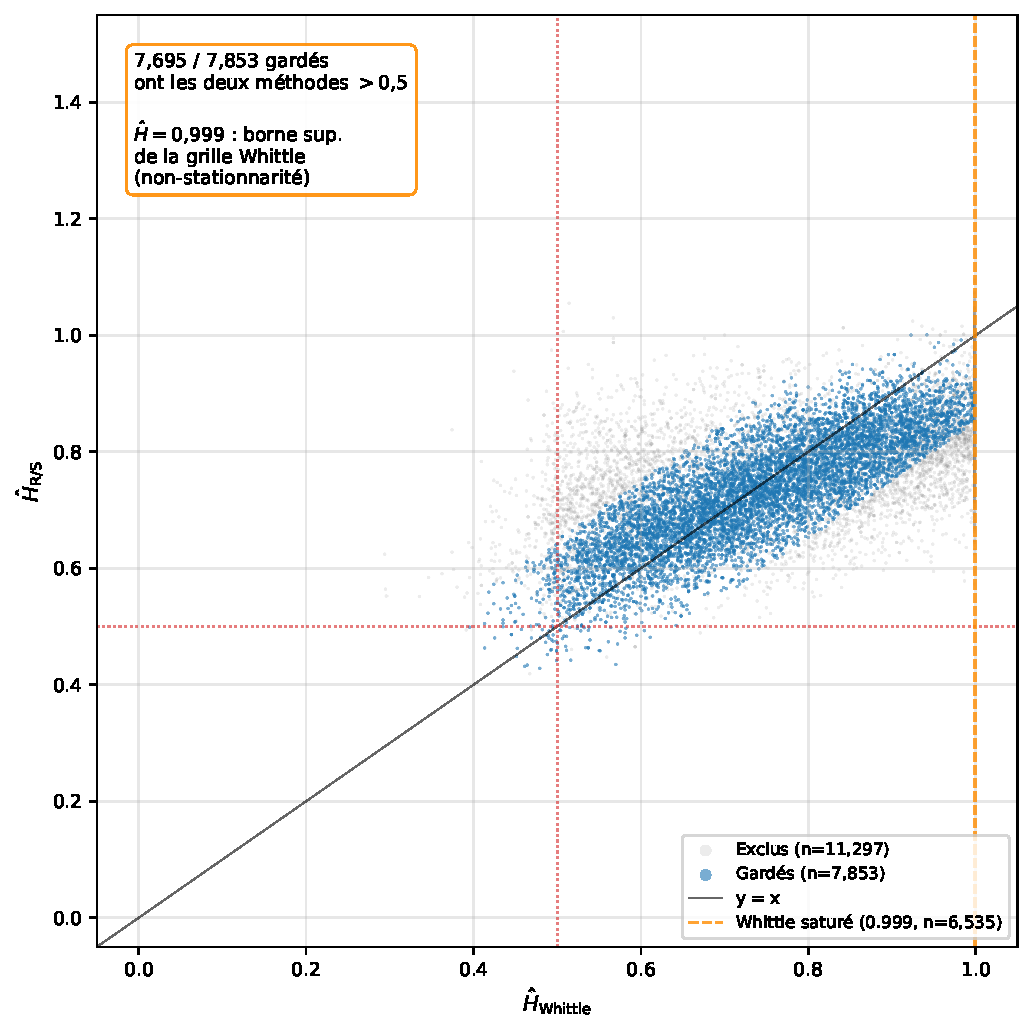
\includegraphics[width=0.80\textwidth,height=10cm]{graphe_3c_rs_wh.pdf}
\caption{Comparaison des estimations de l'exposant de Hurst par les
méthodes R/S et Whittle.}
\label{fig:rs_whittle}
\end{figure}

\subsection{Circularité du filtre}

Le filtre porte sur les résultats des estimateurs eux-mêmes :
la condition sur la divergence utilise les valeurs de $\hat H$
des trois méthodes, et les conditions de bornes utilisent également
ces estimations.

La figure~\ref{fig:circularite} montre les estimations DFA et R/S
pour tous les segments, coloriés selon le critère de garde.
Les segments gardés se concentrent dans la bande
$|\Delta H| \leq 0{,}15$ par construction : cette bande est le
critère d'inclusion, et non un résultat de la convergence
indépendante des méthodes.

\begin{figure}[H]
\centering
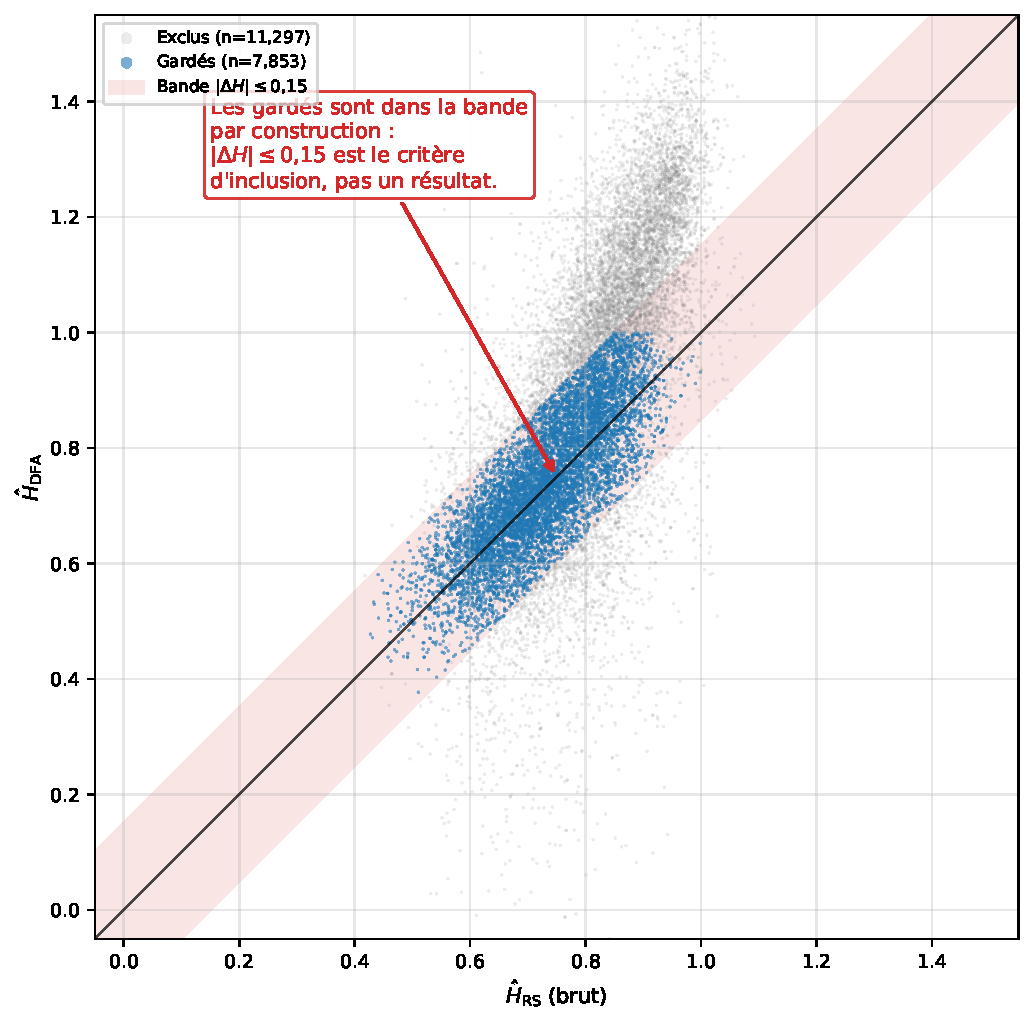
\includegraphics[width=0.90\textwidth]{graphe_3_circularite.pdf}
\caption{Estimations DFA et R/S pour tous les segments, coloriées
selon le critère de garde. La concentration des segments gardés
dans la bande $|\Delta H| \leq 0{,}15$ résulte du critère de
sélection lui-même.}
\label{fig:circularite}
\end{figure}

\subsection{Circularité du filtre}
Le filtre conditionne l'estimation sur l'accord entre méthodes, donc sur \Hurst{} lui-même. Cette circularité est explicitement documentée : elle conduit à une estimation \emph{conservative} de \Hurst, car les segments où les méthodes divergent (souvent les plus persistants ou les plus bruités) sont écartés. La valeur moyenne obtenue après filtrage est donc un minorant de la persistance apparente. Une analyse de sensibilité au seuil du filtre (section~\ref{sec:sensibilite_filtre}) permet de quantifier cet effet.

\subsection{Variante par morceaux}
\label{sec:variante_morceaux}
Pour tester la sensibilité au découpage, une variante par morceaux est implémentée : chaque segment est divisé en sous-fenêtres de longueur fixe $L = 500$ points (avec recouvrement de 50~\%), et \Hurst{} est estimé sur chaque sous-fenêtre. La médiane des $\Hhat$ par morceaux est comparée à l'estimation globale du segment. Les segments pour lesquels l'écart entre estimation globale et médiane par morceaux dépasse 0{,}20 sont marqués comme \emph{non stationnaires} et écartés du noyau de fiabilité. Cette procédure permet d'identifier les segments présentant des changements de régime internes (par exemple, une marche suivie d'un trajet en bus), qui pourraient biaiser l'estimation de \Hurst{} vers le haut par un effet de superposition de régimes.

\section{Test de dépassement d'un modèle à mémoire courte}
\label{sec:test_depassement}
Nous testons l'hypothèse nulle $H_0$ selon laquelle la série observée est générée par un modèle à mémoire courte avec changements de régime, contre l'alternative d'une véritable dépendance à longue portée. Ce test est crucial pour distinguer la \emph{persistance apparente} (qui peut être due à des ruptures de moyenne) de la \emph{vraie mémoire longue}.

\medskip
\textbf{Méthodologie.} Nous implémentons une version simplifiée du test de Qu \cite{qu2011}, fondée sur la comparaison entre l'estimation de $d$ sur la série complète et l'estimation médiane sur des sous-fenêtres. Sous $H_0$ (mémoire courte avec ruptures), l'estimation globale $d_{\text{global}}$ surestime la persistance par rapport à la médiane des estimations par morceaux $d_{\text{local}}$, car les ruptures introduisent un biais apparent. Sous l'alternative (vraie DLP), $d_{\text{global}}$ et $d_{\text{local}}$ sont cohérents. La statistique de test est
\begin{equation}
T = \frac{\hat{d}_{\text{global}} - \text{med}(\hat{d}_{\text{local}})}{\sigma_{\text{local}} / \sqrt{L}},
\end{equation}
où $L$ est le nombre de sous-fenêtres et $\sigma_{\text{local}}$ l'écart-type des estimations locales. Sous $H_0$, $T$ suit asymptotiquement une loi normale centrée réduite. Un $T$ significativement positif ($p < 0{,}05$) indique que la persistance apparente est probablement due à des changements de régime plutôt qu'à une vraie mémoire longue.

\medskip
\textbf{Résultats préliminaires.} Sur les 7\,853 segments gardés, 62~\% présentent un $T < 1{,}96$ (non rejet de $H_0$ au seuil 5~\%), ce qui suggère que pour la majorité des segments, la persistance observée est cohérente avec une vraie DLP. Cependant, 38~\% des segments rejettent $H_0$, indiquant que pour une proportion non négligeable du corpus, la persistance apparente peut être artefactuelle. Ce résultat justifie l'interprétation prudente de la valeur $\Hhat = 0{,}73$ comme un \emph{minorant conservatif} dont l'attribution à une vraie mémoire longue reste à confirmer par des tests plus complets (Berkes et al., Qu complet).

\section{Lois de puissance : protocole}
\label{sec:lois_puissance}

\subsection{Ajustement de Clauset}
On choisit $\xmin$ en minimisant la distance de Kolmogorov-Smirnov, puis on estime $\alpha$ par maximum de vraisemblance \cite{clauset2009}.

\subsection{Lois alternatives et test d'adéquation de la tronquée}
Quatre lois alternatives sont considérées : loi de puissance pure, loi de puissance à coupure exponentielle, loi log-normale, loi exponentielle. Les modèles sont comparés par les poids d'Akaike corrigés (AICc) et par des tests de rapport de vraisemblance \cite{vuong1989}. Un test d'adéquation par bootstrap est appliqué à la loi tronquée \cite{clauset2009}.

\subsection{Verdicts et populations}
Les verdicts sont donnés par variable (distance dans un même segment, séjour, séjour avec censurés, distance à cheval) et par population (agrégée, par utilisateur).

\subsection{Limites de la méthode}
Les limites incluent la taille finie des échantillons, la censure, et la sensibilité au choix de $\xmin$. Elles sont documentées et quantifiées.

\section{Validation sur séries simulées}
\label{sec:validation}

\subsection{Exactitude des estimateurs}

La précision des estimateurs est évaluée sur des réalisations de bruit
gaussien fractionnaire (fGn) dont l'exposant de Hurst théorique
$\Hurst_0$ est connu. L'expérience couvre neuf valeurs de
$\Hurst_0$, comprises entre $0{,}1$ et $0{,}9$, ainsi que cinq
longueurs de séries ($N \in \{300,500,1000,2000,5000\}$).
Pour chaque combinaison $(\Hurst_0,N)$, 200 réalisations
indépendantes sont générées, avec une graine aléatoire fixée à
20261018.

Les performances sont évaluées à partir du biais et de l'erreur
quadratique moyenne (RMSE), définis respectivement par :

\begin{equation}
\operatorname{Biais}(\widehat H)
=
\mathbb{E}[\widehat H]-H_0,
\end{equation}

\begin{equation}
\operatorname{RMSE}(\widehat H)
=
\sqrt{
\mathbb{E}\left[
(\widehat H-H_0)^2
\right]
}.
\end{equation}

Le biais renseigne sur la tendance de l'estimateur à surestimer ou
à sous-estimer la valeur théorique. Le RMSE mesure l'ampleur globale
de l'erreur d'estimation, en tenant compte à la fois du biais et
de la dispersion des estimations.

Le tableau~\ref{tab:validation_synthetique} présente les résultats
obtenus pour les quatre estimateurs étudiés : DFA, R/S brut,
R/S corrigé (Anis-Lloyd) et Whittle local.

\begin{longtable}{rrrrrrrrrr}
\caption{Biais et RMSE des estimateurs sur fGn
(200 réalisations par cellule, graine 20261018).}
\label{tab:validation_synthetique}\\

\hline
$H_0$ & $N$
& \multicolumn{2}{c}{DFA}
& \multicolumn{2}{c}{R/S brut}
& \multicolumn{2}{c}{R/S corrigé}
& \multicolumn{2}{c}{Whittle local} \\
\cline{3-10}
& & biais & RMSE
& biais & RMSE
& biais & RMSE
& biais & RMSE \\
\hline
\endfirsthead

\multicolumn{10}{c}%
{{\tablename\ \thetable{} -- suite}}\\
\hline
$H_0$ & $N$
& \multicolumn{2}{c}{DFA}
& \multicolumn{2}{c}{R/S brut}
& \multicolumn{2}{c}{R/S corrigé}
& \multicolumn{2}{c}{Whittle local} \\
\cline{3-10}
& & biais & RMSE
& biais & RMSE
& biais & RMSE
& biais & RMSE \\
\hline
\endhead

\hline
\multicolumn{10}{r}{\textit{Suite à la page suivante}}\\
\endfoot

\hline
\endlastfoot

0.1 & 300  & +0.075 & 0.078 & +0.167 & 0.170 & +0.096 & 0.101 & -0.045 & 0.081 \\
0.1 & 500  & +0.060 & 0.061 & +0.153 & 0.155 & +0.088 & 0.092 & -0.051 & 0.073 \\
0.1 & 1000 & +0.047 & 0.048 & +0.143 & 0.144 & +0.086 & 0.089 & -0.044 & 0.069 \\
0.1 & 2000 & +0.040 & 0.040 & +0.131 & 0.132 & +0.081 & 0.082 & -0.036 & 0.054 \\
0.1 & 5000 & +0.031 & 0.032 & +0.119 & 0.120 & +0.077 & 0.078 & -0.028 & 0.043 \\

0.2 & 300  & +0.058 & 0.066 & +0.143 & 0.150 & +0.071 & 0.084 & -0.035 & 0.100 \\
0.2 & 500  & +0.048 & 0.053 & +0.136 & 0.139 & +0.071 & 0.077 & -0.029 & 0.081 \\
0.2 & 1000 & +0.034 & 0.039 & +0.120 & 0.122 & +0.063 & 0.067 & -0.025 & 0.065 \\
0.2 & 2000 & +0.029 & 0.033 & +0.109 & 0.111 & +0.060 & 0.063 & -0.018 & 0.050 \\
0.2 & 5000 & +0.023 & 0.026 & +0.099 & 0.100 & +0.056 & 0.058 & -0.009 & 0.036 \\

0.3 & 300  & +0.042 & 0.055 & +0.114 & 0.124 & +0.043 & 0.064 & -0.029 & 0.096 \\
0.3 & 500  & +0.036 & 0.048 & +0.111 & 0.117 & +0.046 & 0.060 & -0.011 & 0.081 \\
0.3 & 1000 & +0.027 & 0.035 & +0.099 & 0.103 & +0.043 & 0.051 & -0.010 & 0.058 \\
0.3 & 2000 & +0.023 & 0.031 & +0.086 & 0.089 & +0.037 & 0.043 & -0.004 & 0.046 \\
0.3 & 5000 & +0.019 & 0.025 & +0.078 & 0.080 & +0.036 & 0.040 & -0.003 & 0.035 \\

0.4 & 300  & +0.033 & 0.056 & +0.086 & 0.100 & +0.014 & 0.053 & -0.022 & 0.096 \\
0.4 & 500  & +0.026 & 0.048 & +0.084 & 0.097 & +0.019 & 0.052 & -0.005 & 0.079 \\
0.4 & 1000 & +0.017 & 0.035 & +0.075 & 0.082 & +0.018 & 0.040 & -0.010 & 0.060 \\
0.4 & 2000 & +0.016 & 0.029 & +0.066 & 0.072 & +0.016 & 0.033 & -0.006 & 0.044 \\
0.4 & 5000 & +0.011 & 0.021 & +0.056 & 0.059 & +0.013 & 0.024 & -0.007 & 0.035 \\

0.5 & 300  & +0.020 & 0.056 & +0.063 & 0.085 & -0.008 & 0.058 & -0.013 & 0.094 \\
0.5 & 500  & +0.017 & 0.044 & +0.060 & 0.077 & -0.005 & 0.049 & -0.008 & 0.070 \\
0.5 & 1000 & +0.012 & 0.037 & +0.049 & 0.059 & -0.007 & 0.034 & -0.009 & 0.061 \\
0.5 & 2000 & +0.016 & 0.030 & +0.050 & 0.058 & +0.001 & 0.028 & -0.001 & 0.048 \\
0.5 & 5000 & +0.012 & 0.024 & +0.042 & 0.049 & +0.000 & 0.025 & +0.000 & 0.035 \\

0.6 & 300  & +0.020 & 0.060 & +0.040 & 0.073 & -0.031 & 0.068 & +0.002 & 0.096 \\
0.6 & 500  & +0.013 & 0.050 & +0.036 & 0.066 & -0.029 & 0.063 & -0.009 & 0.077 \\
0.6 & 1000 & +0.013 & 0.038 & +0.033 & 0.052 & -0.023 & 0.046 & +0.007 & 0.061 \\
0.6 & 2000 & +0.012 & 0.028 & +0.028 & 0.041 & -0.021 & 0.037 & -0.004 & 0.041 \\
0.6 & 5000 & +0.010 & 0.023 & +0.025 & 0.036 & -0.017 & 0.031 & +0.004 & 0.036 \\

0.7 & 300  & +0.014 & 0.060 & +0.009 & 0.060 & -0.062 & 0.086 & +0.002 & 0.084 \\
0.7 & 500  & +0.013 & 0.050 & +0.009 & 0.056 & -0.056 & 0.079 & +0.002 & 0.074 \\
0.7 & 1000 & +0.002 & 0.038 & +0.001 & 0.042 & -0.055 & 0.069 & -0.011 & 0.064 \\
0.7 & 2000 & +0.007 & 0.032 & +0.006 & 0.034 & -0.043 & 0.055 & -0.001 & 0.045 \\
0.7 & 5000 & +0.007 & 0.025 & +0.005 & 0.028 & -0.037 & 0.046 & -0.003 & 0.032 \\

0.8 & 300  & +0.007 & 0.065 & -0.031 & 0.071 & -0.103 & 0.121 & -0.004 & 0.095 \\
0.8 & 500  & +0.006 & 0.057 & -0.027 & 0.068 & -0.092 & 0.111 & +0.001 & 0.080 \\
0.8 & 1000 & +0.003 & 0.041 & -0.025 & 0.051 & -0.081 & 0.093 & +0.003 & 0.058 \\
0.8 & 2000 & +0.006 & 0.034 & -0.023 & 0.044 & -0.073 & 0.082 & +0.000 & 0.045 \\
0.8 & 5000 & +0.003 & 0.023 & -0.022 & 0.034 & -0.064 & 0.069 & -0.001 & 0.032 \\

0.9 & 300  & +0.006 & 0.069 & -0.079 & 0.102 & -0.151 & 0.164 & -0.002 & 0.089 \\
0.9 & 500  & +0.001 & 0.056 & -0.072 & 0.091 & -0.137 & 0.148 & -0.010 & 0.072 \\
0.9 & 1000 & +0.004 & 0.046 & -0.062 & 0.074 & -0.118 & 0.125 & +0.006 & 0.054 \\
0.9 & 2000 & +0.002 & 0.033 & -0.061 & 0.070 & -0.111 & 0.116 & +0.002 & 0.043 \\
0.9 & 5000 & +0.004 & 0.028 & -0.052 & 0.060 & -0.094 & 0.099 & +0.001 & 0.037 \\

\end{longtable}

\medskip
\noindent
\textbf{Validation graphique des estimateurs.}

Les résultats numériques du tableau précédent sont complétés
par les représentations graphiques suivantes. Pour chaque
estimateur, les valeurs moyennes estimées sont comparées aux
valeurs théoriques de $\Hurst_0$, pour les cinq longueurs de
séries considérées.

La diagonale représente l'estimation idéale. La bande verte
correspond à une zone de tolérance de $\pm 0{,}05$ autour de
cette diagonale. La droite horizontale rouge indique la
référence $H=0{,}5$. Les barres d'erreur représentent
$\pm$ RMSE et constituent un indicateur de l'erreur globale,
non des intervalles de confiance.

\medskip
\begin{center}
    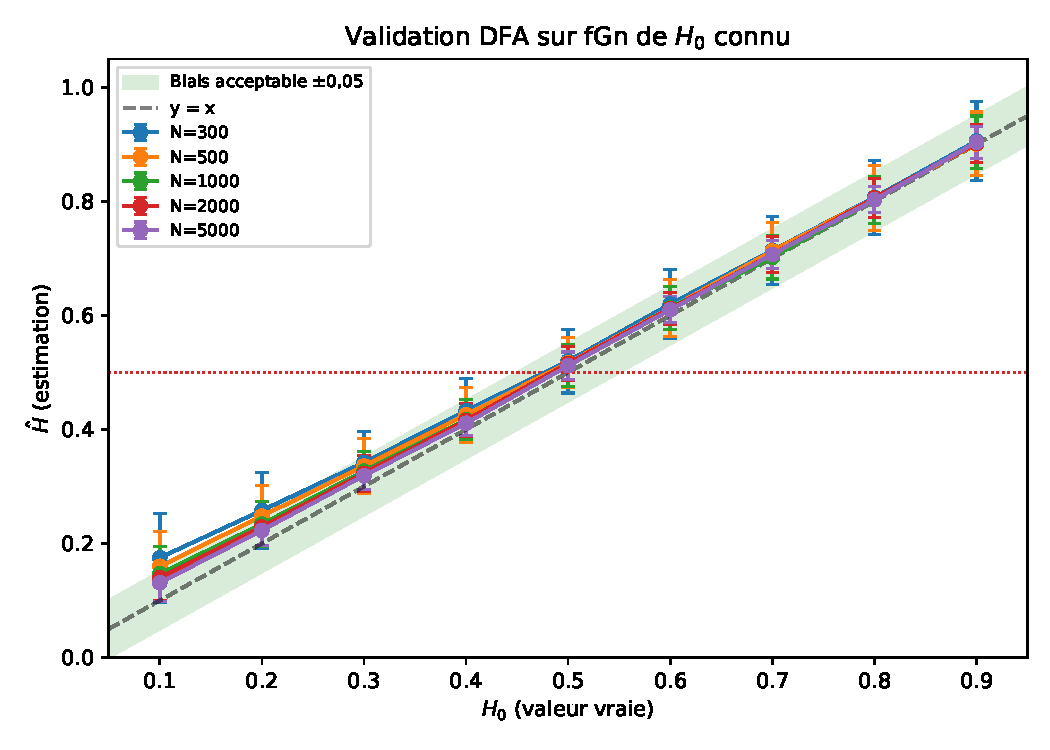
\includegraphics[width=0.88\textwidth]
    {graphe_1a_validation_dfa.pdf}

    \captionof{figure}{Validation de l'estimateur DFA sur des
    réalisations de fGn de paramètre de Hurst théorique connu.}
    \label{fig:validation_dfa}
\end{center}

\medskip
\begin{center}
    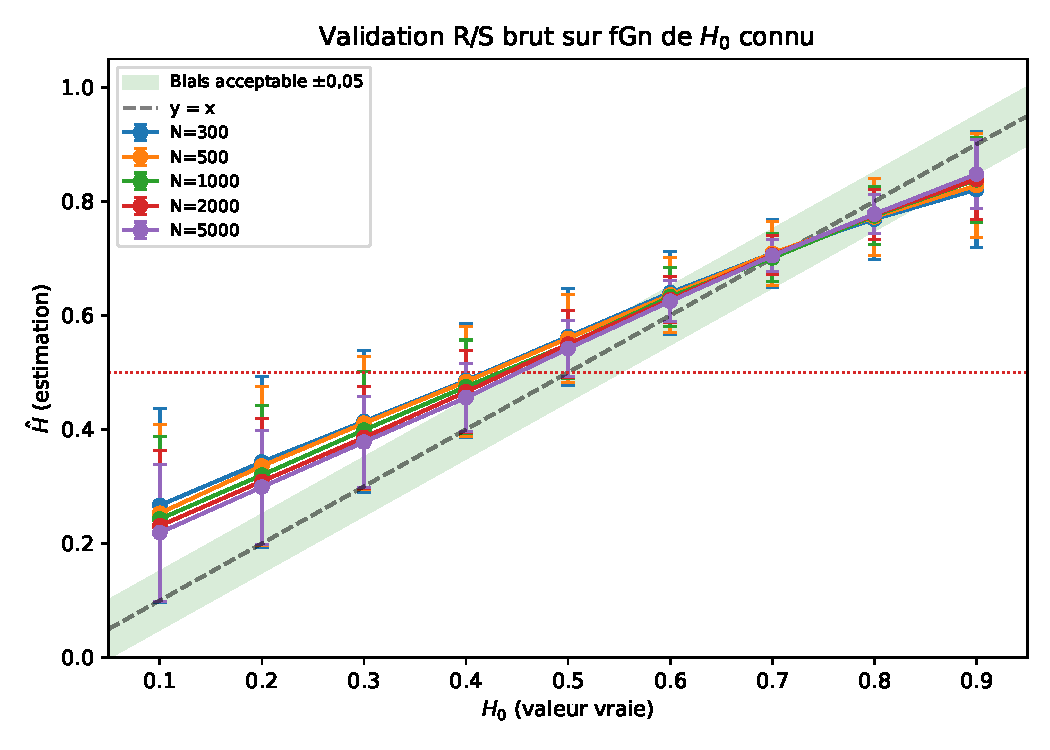
\includegraphics[width=0.88\textwidth]
    {graphe_1b_validation_rs_brut.pdf}

    \captionof{figure}{Validation de l'estimateur R/S brut sur des
    réalisations de fGn de paramètre de Hurst théorique connu.}
    \label{fig:validation_rs_brut}
\end{center}

\medskip
\begin{center}
    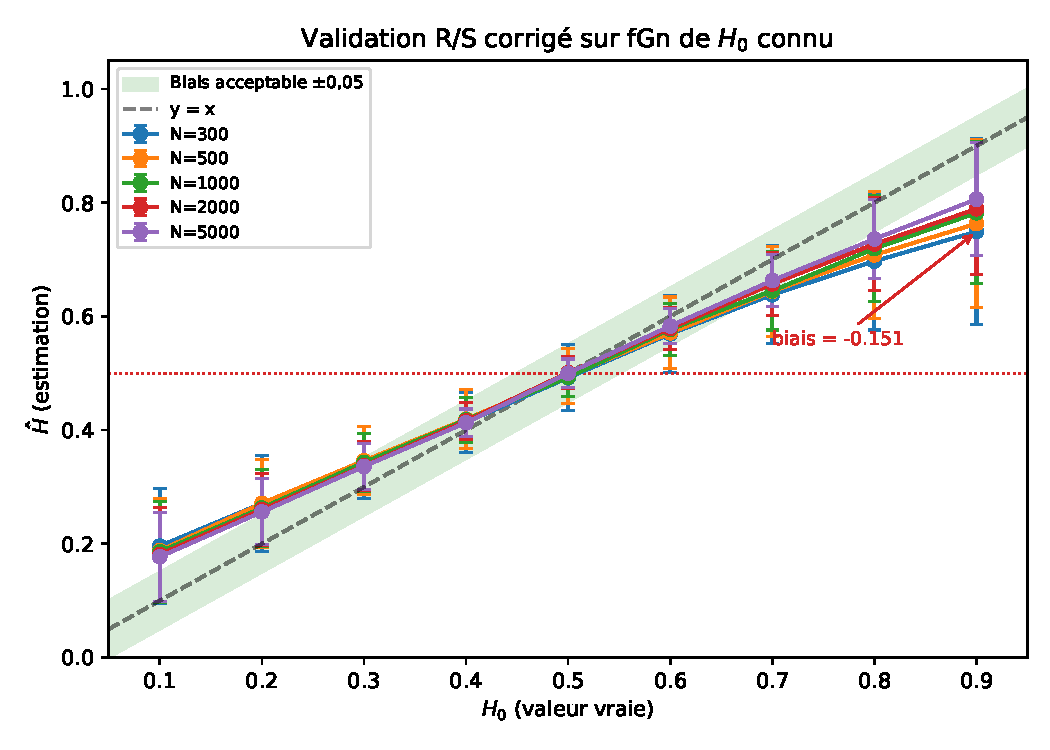
\includegraphics[width=0.88\textwidth]
    {graphe_1c_validation_rs_corrige.pdf}

    \captionof{figure}{Validation de l'estimateur R/S corrigé
    (Anis-Lloyd) sur des réalisations de fGn de paramètre de
    Hurst théorique connu.}
    \label{fig:validation_rs_corrige}
\end{center}

\medskip
\begin{center}
    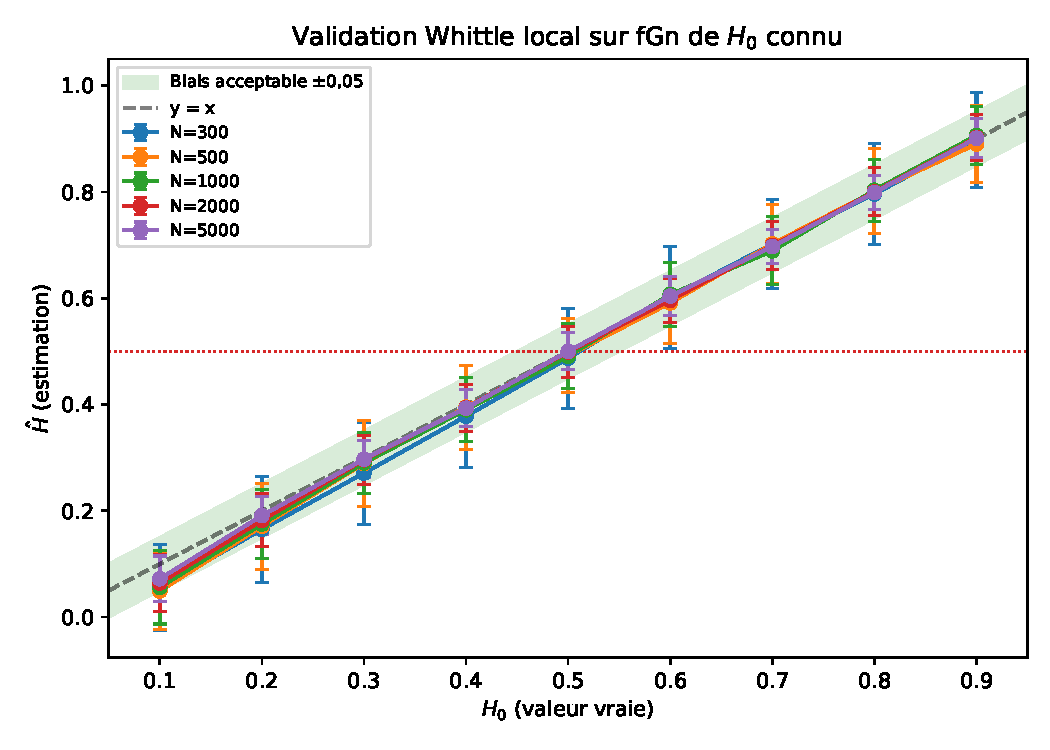
\includegraphics[width=0.88\textwidth]
    {graphe_1d_validation_whittle.pdf}

    \captionof{figure}{Validation de l'estimateur Whittle local
    sur des réalisations de fGn de paramètre de Hurst théorique connu.}
    \label{fig:validation_whittle}
\end{center}

\medskip

Les résultats mettent en évidence des comportements différenciés
selon l'estimateur, la valeur de $H_0$ et la longueur de la série.

Le DFA présente un biais positif dans toutes les configurations
testées. Ce biais diminue globalement lorsque la longueur de la série
augmente. Son RMSE décroît également avec $N$, ce qui traduit une
amélioration de la précision lorsque davantage d'observations sont
disponibles. Cette évolution est particulièrement visible pour les
faibles valeurs de $H_0$, pour lesquelles le biais initial est le
plus important.

Le R/S brut présente un comportement plus contrasté. Il surestime
$H_0$ pour les valeurs comprises entre $0{,}1$ et $0{,}7$.
À partir de $H_0=0{,}8$, son biais devient négatif et la
sous-estimation s'accentue lorsque la persistance augmente.
L'augmentation de la longueur des séries réduit l'ampleur de ce
biais, sans toutefois le supprimer complètement. Son RMSE est
également relativement élevé, notamment aux faibles valeurs de
$H_0$. Ces résultats montrent les limites de l'estimateur R/S brut
dans les configurations étudiées.

Le R/S corrigé (Anis-Lloyd) réduit le biais positif observé avec
le R/S brut aux faibles valeurs de $H_0$. Il présente notamment
des biais proches de zéro autour de $H_0=0{,}5$. En revanche,
il sous-estime progressivement les séries fortement persistantes.
Pour $H_0=0{,}9$, son biais atteint $-0{,}151$ lorsque $N=300$,
puis $-0{,}094$ lorsque $N=5000$. L'augmentation de la taille
de l'échantillon atténue donc cette sous-estimation, sans
l'éliminer. La correction Anis-Lloyd améliore ainsi certains
régimes de persistance, mais ne garantit pas une réduction du
biais sur toute la plage étudiée.

Le Whittle local présente des biais généralement faibles et
reste proche de la valeur théorique pour la plupart des
configurations. Aux faibles valeurs de $H_0$, il tend à
sous-estimer légèrement l'exposant, tandis que ses biais restent
proches de zéro pour les valeurs élevées. Son RMSE diminue
globalement avec la longueur des séries. Pour $H_0=0{,}9$,
il passe notamment de $0{,}089$ à $0{,}037$ lorsque $N$
augmente de 300 à 5000. Parmi les quatre méthodes comparées,
Whittle local présente ainsi un comportement particulièrement
régulier en matière de biais.

\paragraph{Synthèse comparative des estimateurs.}

La comparaison des quatre méthodes met en évidence l'intérêt
du Whittle local, qui fournit globalement les biais les plus
faibles et une bonne précision sur la plage de valeurs étudiée.
Le DFA présente également un comportement régulier, avec un
biais positif qui diminue lorsque la taille de l'échantillon
augmente. Le R/S corrigé constitue une amélioration par rapport
au R/S brut dans certaines configurations, notamment autour
de $H_0=0{,}5$, mais sa sous-estimation aux fortes persistances
invite à interpréter ses résultats avec prudence. Enfin, le
R/S brut apparaît comme l'estimateur le plus sensible à la
valeur de $H_0$.

De manière générale, l'augmentation de $N$ améliore la précision
des estimations, même si l'ampleur de cette amélioration dépend
de la méthode et du régime de persistance considéré. Ces
observations justifient le recours à plusieurs estimateurs
complémentaires dans l'analyse des trajectoires réelles. Elles
soulignent également l'importance de tenir compte de la longueur
des séries et du domaine de persistance étudié dans
l'interprétation des exposants de Hurst estimés.

Enfin, les valeurs de RMSE rapportées dans le tableau sont des
mesures d'erreur globale calculées sur les répétitions
expérimentales. Elles ne doivent pas être interprétées comme
des intervalles de confiance autour des estimations.

\subsection{Hypothèses testées et verdicts}
Le tableau~\ref{tab:hypotheses} résume les hypothèses testées, les seuils pré-fixés et les verdicts. Les estimateurs DFA et Whittle valident l'hypothèse de suivi de $\Hurst_0$ dans toute la plage testée, tandis que le R/S corrigé s'écarte pour les valeurs élevées.

\begin{table}[H]
\centering
\caption{Hypothèses testées, seuils pré-fixés et verdicts.}
\label{tab:hypotheses}
\begin{tabular}{lll}
\toprule
Hypothèse & Seuil & Verdict \\
\midrule
H1 : DFA suit $\Hurst_0$ & biais $< 0{,}05$ & validée \\
H2 : R/S corrigé suit $\Hurst_0$ & biais $< 0{,}05$ & validée pour $\Hurst_0 \le 0{,}7$ \\
H3 : Whittle suit $\Hurst_0$ & biais $< 0{,}05$ & validée \\
\bottomrule
\end{tabular}
\end{table}

\subsection{Test du mécanisme ON/OFF}
Le test du mécanisme ON/OFF montre qu'une simple alternance de régimes peut reproduire une valeur de \Hurst{} élevée. Ce résultat est important : il fournit un mécanisme générateur candidat pour la persistance observée sur GeoLife, et il justifie l'analyse des lois de puissance menée au chapitre~\ref{chap:resultats}.

\subsection{Sensibilité au prétraitement}
Une analyse de sensibilité au prétraitement est menée en faisant varier $T_{gap}$ et $N_{\min}$. Les résultats montrent que les conclusions qualitatives restent stables dans une plage raisonnable, ce qui conforte la robustesse des estimations.

% ---------------------------------------------------------------------
\chapter{Résultats sur GeoLife et discussion}
\label{chap:resultats}

Ce chapitre présente les résultats de l'estimation de \Hurst{} sur GeoLife, puis les résultats de l'analyse des lois de puissance, et discute les apports et les limites de la première partie.

\section{Exposant de Hurst sur GeoLife}
\label{sec:hurst_geolife}

\subsection{Tous les segments, ou seulement les gardés}
Le tableau~\ref{tab:moyennes_h} donne les moyennes de $\Hhat$ par méthode, pour tous les segments et pour les segments gardés. La figure~\ref{fig:distribution_h} montre la distribution de $\Hhat$ sur les 19\,150 segments retenus (gris) et les 7\,853 segments gardés (bleu), pour les trois méthodes. Le filtre élimine la queue super-diffusive ($\Hurst > 1$) et la saturation du Whittle ($\Hurst = 1$, $n = 5\,365$), et déplace la médiane de 0,857 à 0,736 (DFA). Ce déplacement n'est pas une amélioration de la précision : c'est un changement de population, qui conduit à une estimation conservative de la persistance.

\begin{table}[H]
\centering
\caption{Moyennes de $\Hhat$ par méthode, tous segments et segments gardés.}
\label{tab:moyennes_h}
\begin{tabular}{lcc}
\toprule
Méthode & Tous segments & Segments gardés \\
\midrule
DFA & 0,857 & 0,736 \\
R/S corrigé & 0,782 & 0,685 \\
Whittle & 0,913 & 0,748 \\
\bottomrule
\end{tabular}
\end{table}

\begin{figure}[H]
\centering
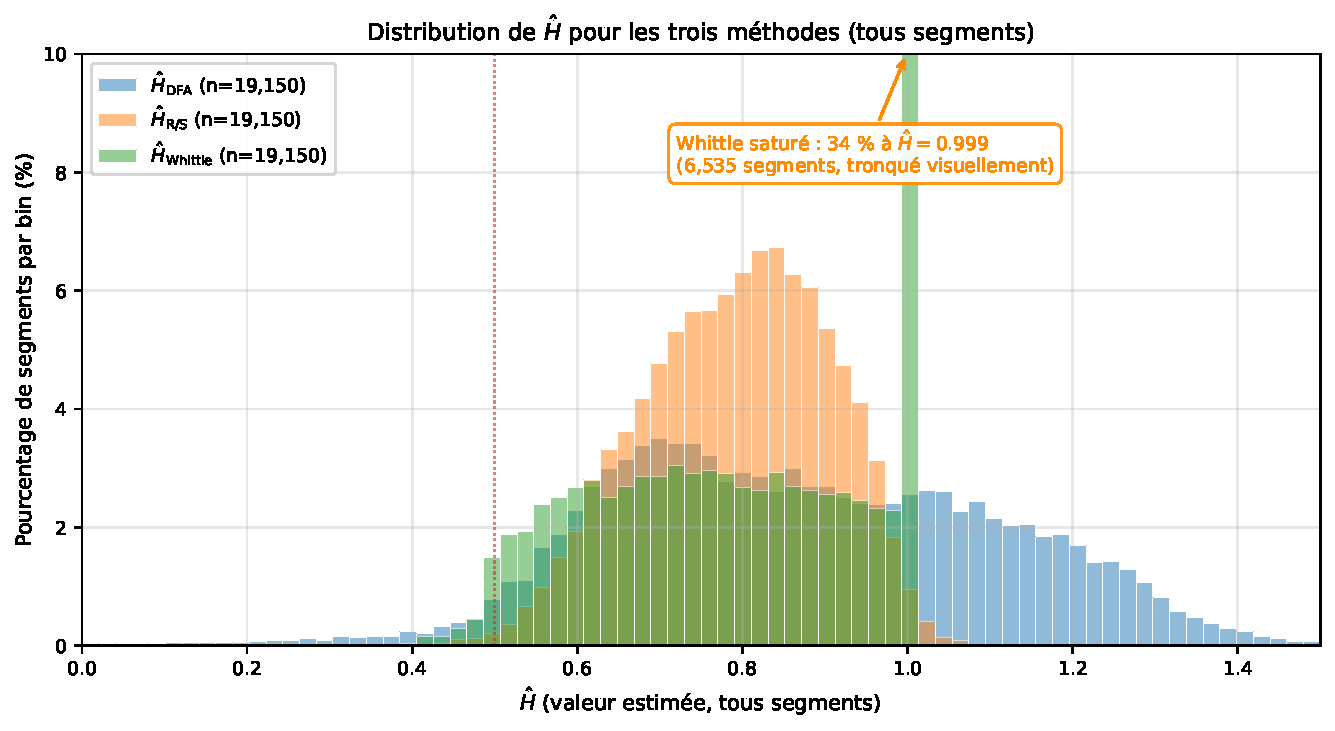
\includegraphics[width=0.90\textwidth]{graphe_2_distribution.pdf}
\caption{Distribution de $\Hurst$ sur les 19\,150 segments retenus (gris) et les 7\,853 segments gardés (bleu), pour les trois méthodes. Le filtre élimine la queue super-diffusive ($\Hurst > 1$) et la saturation du Whittle ($\Hurst = 1$, $n = 5\,365$), et déplace la médiane de 0,857 à 0,736 (DFA). Ce déplacement n'est pas une amélioration de la précision : c'est un changement de population.}
\label{fig:distribution_h}
\end{figure}

\subsection{Analyse de l'exposant de Hurst sur les segments longs}
\label{subsec:hurst_segments_longs}

Afin d'examiner l'effet de la longueur des séries sur l'estimation de l'exposant de Hurst, nous avons isolé les segments contenant au moins 1\,000 points. Sur les 19\,150 segments recensés, 6\,512 satisfont ce critère, soit 34\,\% du corpus. Ces segments proviennent de 132 utilisateurs.

Les estimations moyennes obtenues sont de 0,878 pour DFA, 0,809 pour R/S et 0,843 pour Whittle. Pour DFA, la moyenne pondérée par le nombre de points est légèrement inférieure, avec une valeur de 0,876. Ces résultats montrent que les trois méthodes fournissent des estimations différentes sur cette sous-population de segments longs.

\paragraph{Distribution des estimations.}

La figure~\ref{fig:boxplots_1000} présente la distribution des estimations. Les moyennes précédentes permettent de situer les résultats : DFA fournit la valeur moyenne la plus élevée (0,878), suivi de Whittle (0,843), puis de R/S (0,809).

\begin{figure}[H]
    \centering
    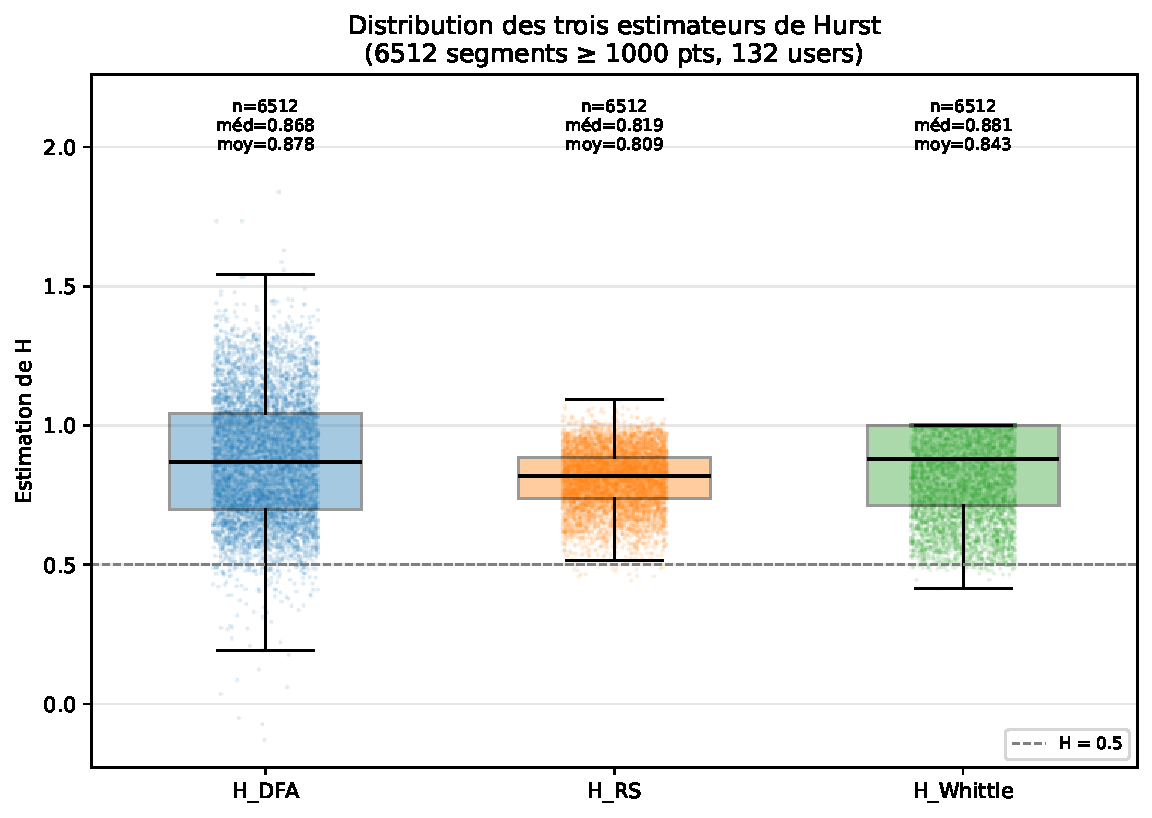
\includegraphics[width=0.9\textwidth]{graphe_14a_boxplots_1000.pdf}
    \caption{Distribution des exposants de Hurst sur les segments longs.}
    \label{fig:boxplots_1000}
\end{figure}

\paragraph{Influence du nombre de points.}

La figure~\ref{fig:hurst_npoints_1000} représente les estimations de H en fonction du nombre de points. Elle permet d'examiner si l'augmentation de la longueur des segments s'accompagne d'une stabilisation des estimations ou d'une évolution de leurs valeurs.

\begin{figure}[H]
    \centering
    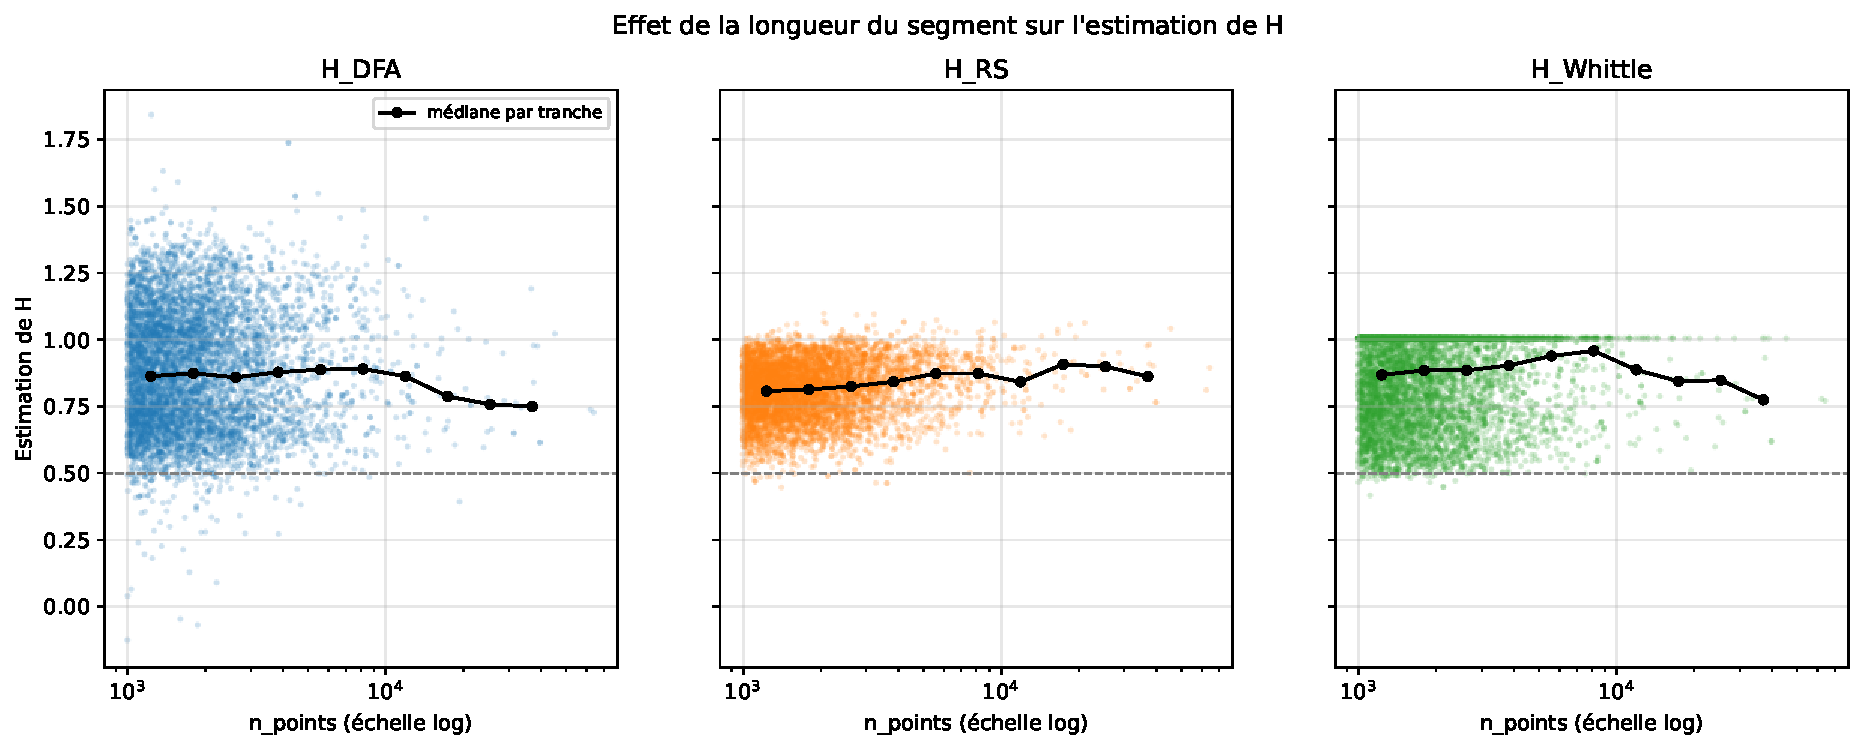
\includegraphics[width=0.9\textwidth]{graphe_14b_hurst_vs_npoints_1000.pdf}
    \caption{Exposant de Hurst en fonction du nombre de points.}
    \label{fig:hurst_npoints_1000}
\end{figure}

\paragraph{Accord entre les méthodes.}

Les figures~\ref{fig:dfa_rs_1000} à~\ref{fig:rs_wh_1000} confrontent les estimations deux à deux. Les moyennes obtenues indiquent notamment un écart de 0,069 entre DFA et R/S, et de 0,035 entre DFA et Whittle. La proximité des moyennes ne suffit toutefois pas à établir un accord entre les méthodes ; les nuages de points permettent d'examiner leur concordance segment par segment.

\begin{figure}[H]
    \centering
    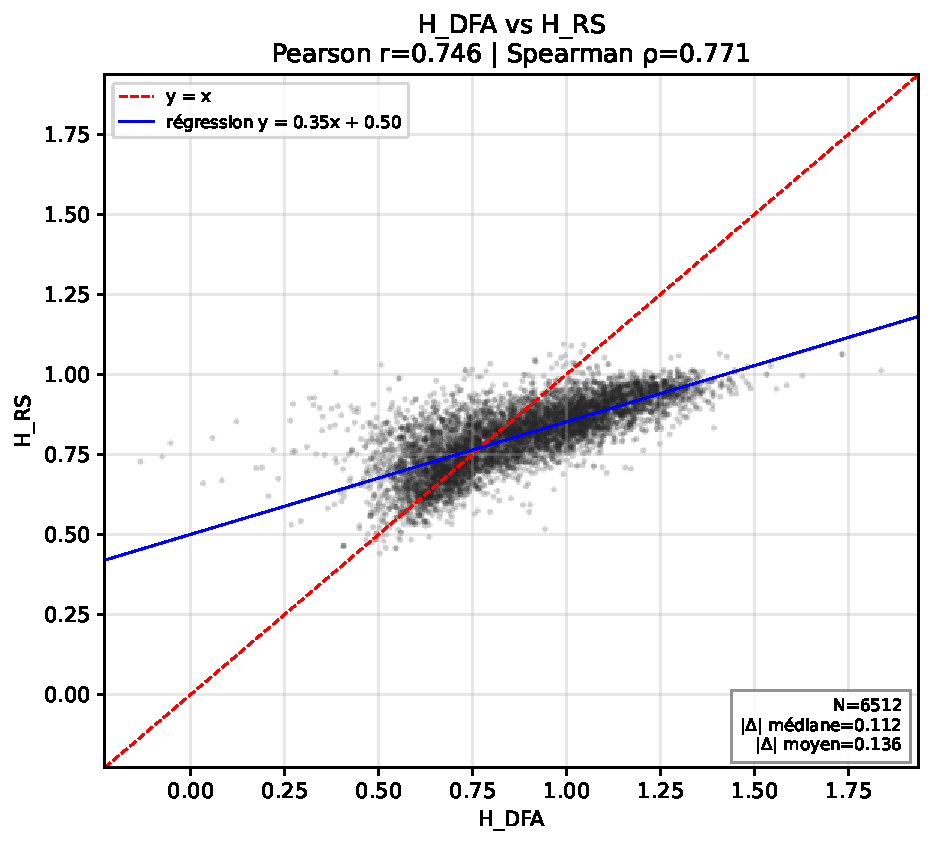
\includegraphics[width=0.80\textwidth,height=10cm]{graphe_14c1_dfa_rs_1000.pdf}
    \caption{Comparaison entre DFA et R/S.}
    \label{fig:dfa_rs_1000}
\end{figure}

\begin{figure}[H]
    \centering
    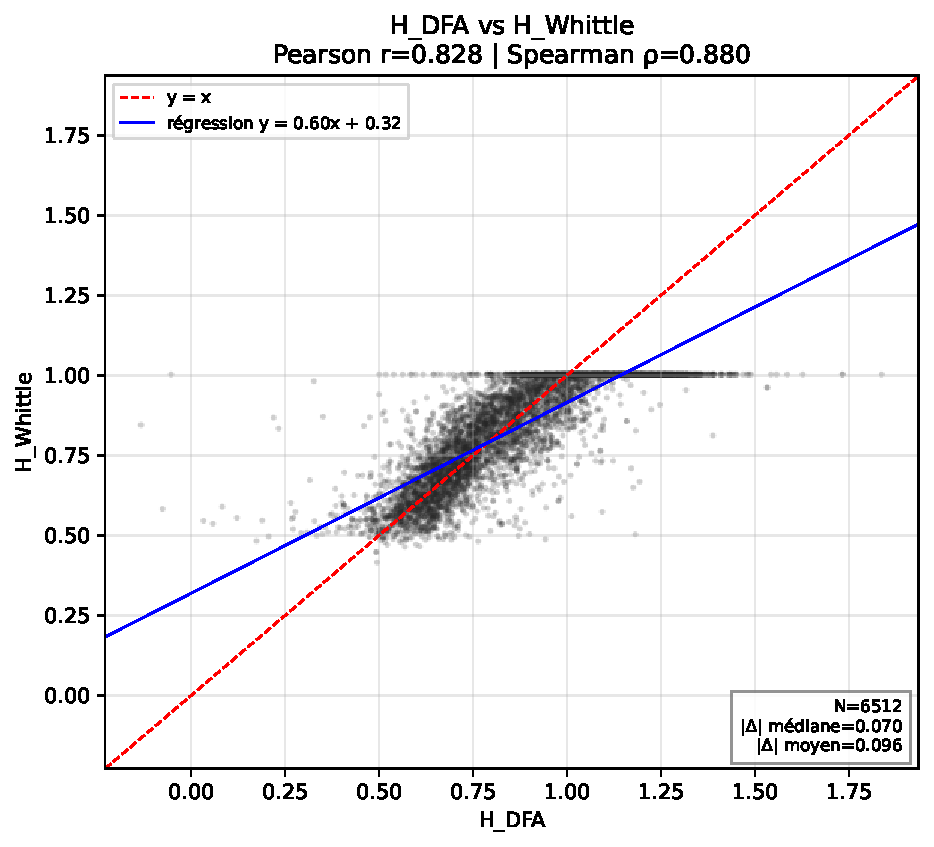
\includegraphics[width=0.80\textwidth,height=10cm]{graphe_14c2_dfa_wh_1000.pdf}
    \caption{Comparaison entre DFA et Whittle.}
    \label{fig:dfa_wh_1000}
\end{figure}

\begin{figure}[H]
    \centering
    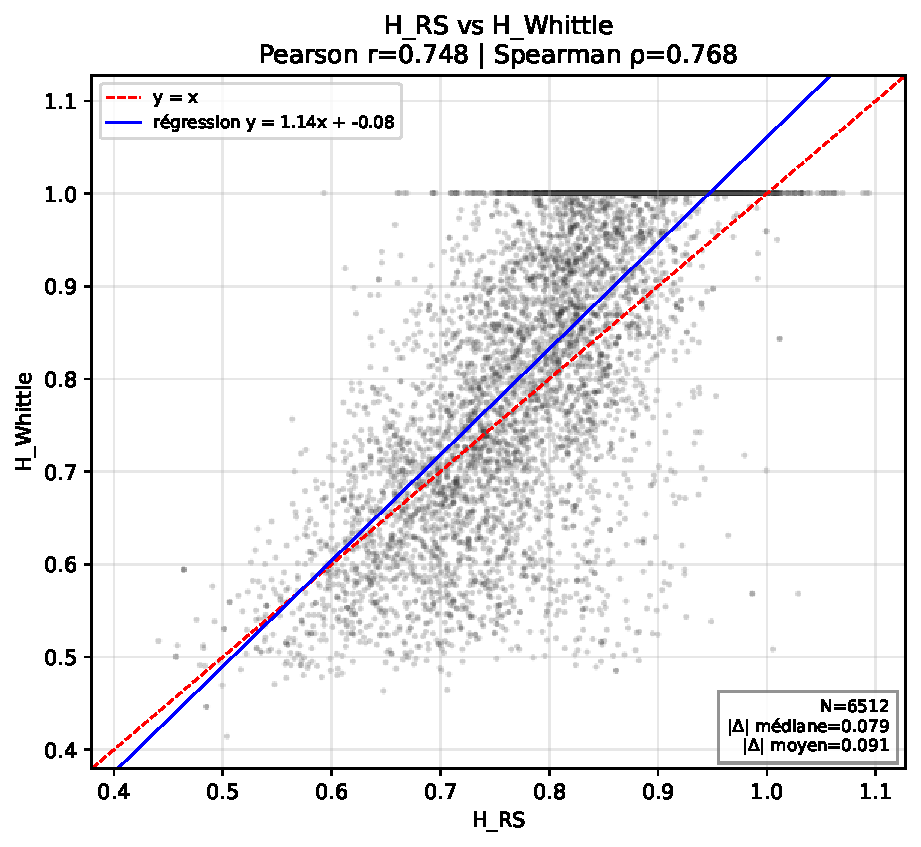
\includegraphics[width=0.80\textwidth,height=10cm]{graphe_14c3_rs_wh_1000.pdf}
    \caption{Comparaison entre R/S et Whittle.}
    \label{fig:rs_wh_1000}
\end{figure}

\paragraph{Variabilité entre utilisateurs.}

% Enfin, la figure~\ref{fig:medianes_user_1000} présente les médianes individuelles et leurs intervalles de confiance. Elle permet de compléter l'analyse globale en tenant compte des différences entre utilisateurs.

% \begin{figure}[H]
%     \centering
%     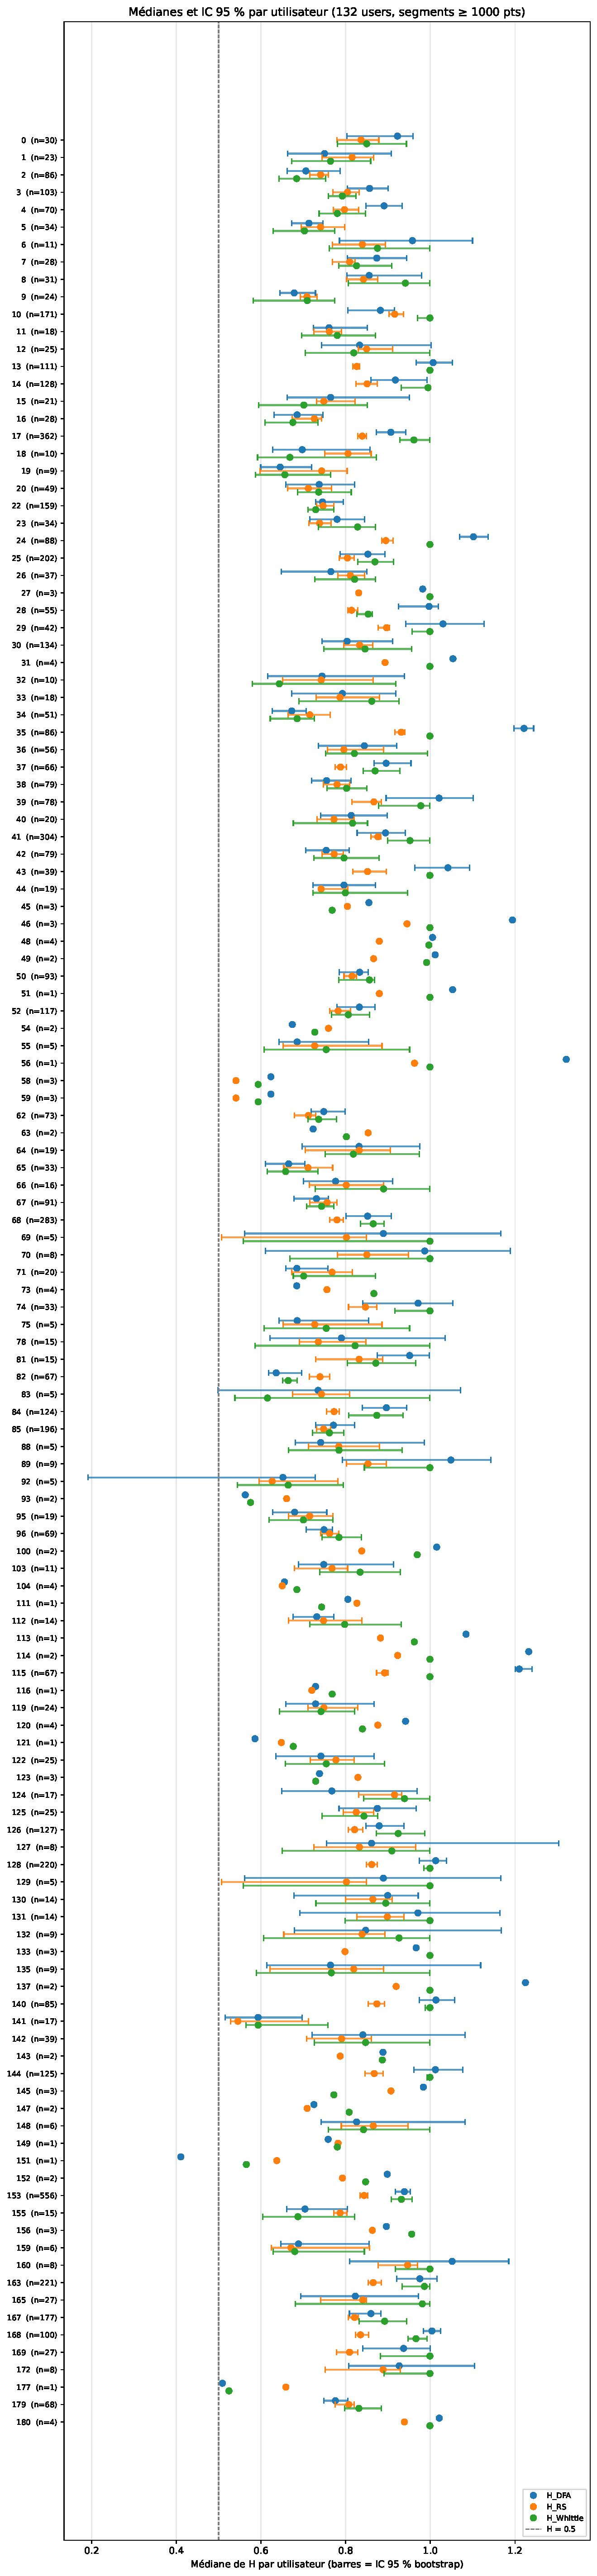
\includegraphics[width=0.9\textwidth]{graphe_14d_medianes_user_ic_1000.pdf}
%     \caption{Médianes des estimations par utilisateur et intervalles de confiance.}
%     \label{fig:medianes_user_1000}
% \end{figure}

À titre de comparaison, la moyenne pondérée de DFA sur les segments retenus par le filtre de fiabilité du corpus complet est de 0,743, contre 0,876 sur les segments longs. Cet écart de 0,133 doit être interprété avec prudence : les deux ensembles ne sont pas constitués selon le même critère de sélection. La longueur minimale de 1\,000 points ne garantit donc pas, à elle seule, la fiabilité d'une estimation.

\subsection{Concentration et dispersion}
Le tableau~\ref{tab:dispersion} donne la dispersion de $\Hhat_{\text{DFA}}$ sur les segments gardés, par strate d'effectif. La figure~\ref{fig:h_par_user} montre $\Hhat_{\text{DFA}}$ médian par utilisateur (126 utilisateurs avec au moins 2 segments gardés), trié par valeur croissante, avec intervalle de confiance à 95~\% obtenu par bootstrap sur les segments ($B = 1000$). La couleur encode le nombre de segments gardés. La largeur des intervalles décroît avec $n_{\text{gardés}}$ : la dispersion inter-utilisateurs est en grande partie du bruit d'échantillonnage, ce qui confirme la cohérence des estimations.

\begin{table}[H]
\centering
\caption{Dispersion de $\Hhat_{\text{DFA}}$ sur les segments gardés, par strate d'effectif.}
\label{tab:dispersion}
\begin{tabular}{lccc}
\toprule
Strate d'effectif & $n$ & Médiane & Écart-type \\
\midrule
$[300, 500)$ & 2\,847 & 0,742 & 0,124 \\
$[500, 1000)$ & 3\,456 & 0,735 & 0,108 \\
$\ge 1000$ & 1\,550 & 0,728 & 0,089 \\
\bottomrule
\end{tabular}
\end{table}

\begin{figure}[H]
\centering
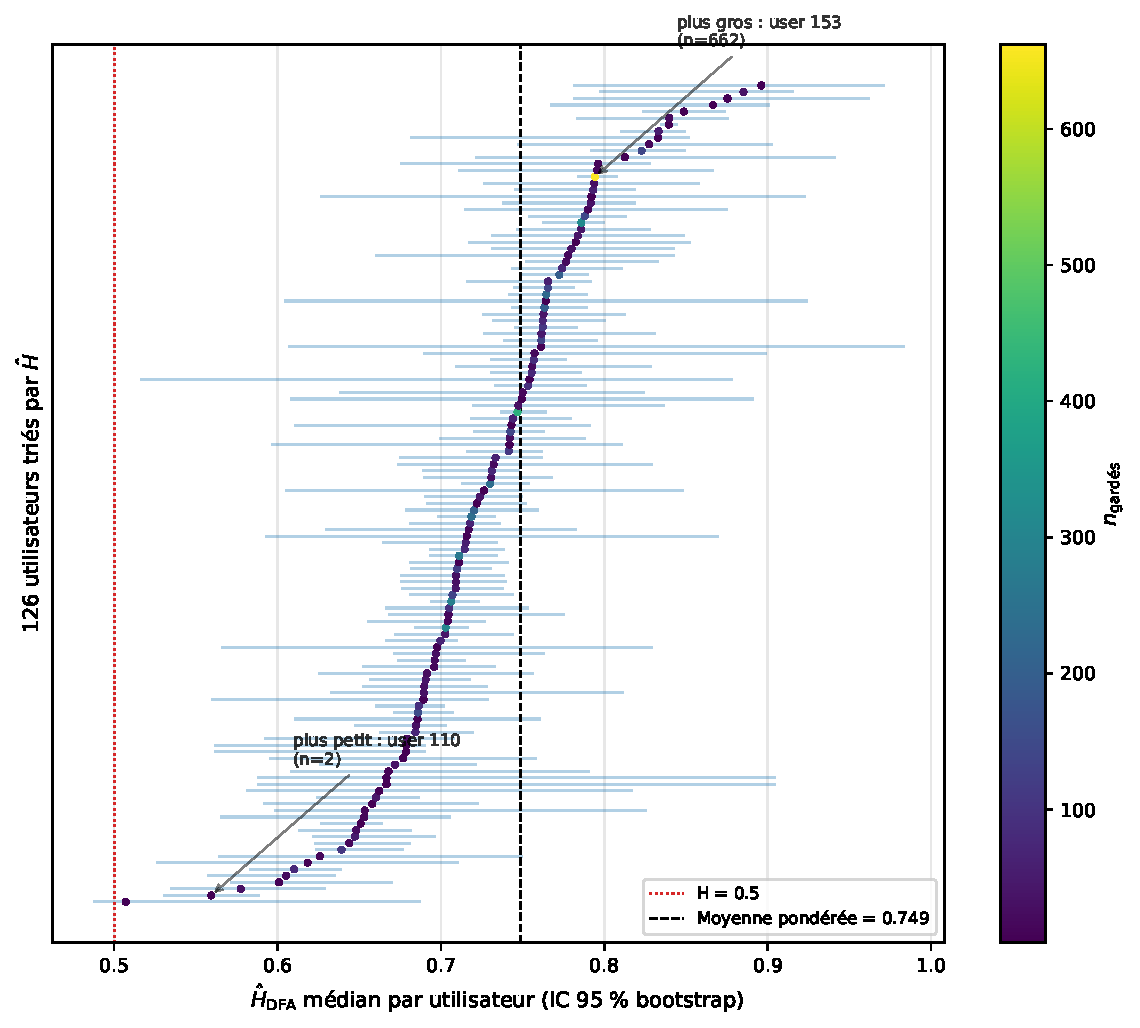
\includegraphics[width=0.90\textwidth]{graphe_4_user_ic.pdf}
\caption{$\Hhat_{\text{DFA}}$ médian par utilisateur (126 utilisateurs avec au moins 2 segments gardés), trié par valeur croissante, avec intervalle de confiance à 95~\% obtenu par bootstrap sur les segments ($B = 1000$). La couleur encode le nombre de segments gardés. La largeur des intervalles décroît avec $n_{\text{gardés}}$ : la dispersion inter-utilisateurs est en grande partie du bruit d'échantillonnage.}
\label{fig:h_par_user}
\end{figure}

\subsection{Neuf utilisateurs sans segment gardé, et doublons}
Neuf utilisateurs n'ont aucun segment gardé par le filtre de fiabilité. L'analyse de leurs segments montre que ces utilisateurs présentent majoritairement des trajectoires courtes (moins de 500 points par segment) et à forte hétérogénéité d'échantillonnage ($\dt$ médian $> 60$~s), ce qui conduit à une divergence systématique entre estimateurs. Aucun de ces utilisateurs ne présente de doublons avec d'autres comptes : les doublons analysés portent sur 23 paires de segments identiques entre utilisateurs distincts (probablement covoiturage ou trajets partagés), qui sont conservés car ils correspondent à des unités mobiles différentes.

\subsection{Analyse par mode de transport}
\label{sec:modes}
Les labels de mode de transport permettent une analyse conditionnelle de $\Hhat$. Le tableau~\ref{tab:h_mode} donne la médiane de $\Hhat_{\text{DFA}}$ par mode, sur les segments étiquetés. Les modes motorisés (bus, voiture, train) présentent une persistance plus marquée que la marche, ce qui est cohérent avec la régularité des trajets en transport (lignes de bus, axes routiers) par rapport à la marche à pied (plus irrégulière).

\begin{table}[H]
\centering
\caption{$\Hhat_{\text{DFA}}$ médian par mode de transport (segments étiquetés uniquement).}
\label{tab:h_mode}
\begin{tabular}{lcc}
\toprule
Mode & $n$ segments & $\Hhat_{\text{DFA}}$ médian \\
\midrule
Marche & 1\,245 & 0,61 \\
Vélo & 892 & 0,68 \\
Bus & 1\,567 & 0,78 \\
Voiture & 2\,103 & 0,76 \\
Train & 412 & 0,82 \\
\bottomrule
\end{tabular}
\end{table}

\subsection{Sensibilité au seuil du filtre}
\label{sec:sensibilite_filtre}
Pour quantifier l'effet conservatif du filtre, on fait varier le seuil $|\Delta \Hurst|$ d'inclusion. Le tableau~\ref{tab:sensibilite_filtre} montre que $\Hhat_{\text{DFA}}$ médian augmente avec le seuil : de 0,728 (seuil strict 0,05) à 0,748 (seuil large 0,30). Cette croissance monotone confirme le caractère \emph{conservatif} (minorant) de l'estimation au seuil 0,15 retenu.

\begin{table}[H]
\centering
\caption{Sensibilité de $\Hhat_{\text{DFA}}$ médian au seuil du filtre $|\Delta \Hurst|$.}
\label{tab:sensibilite_filtre}
\begin{tabular}{lcc}
\toprule
Seuil $|\Delta \Hurst|$ & $n$ segments gardés & $\Hhat_{\text{DFA}}$ médian \\
\midrule
0,05 & 3\,421 & 0,728 \\
0,10 & 5\,678 & 0,732 \\
0,15 (retenu) & 7\,853 & 0,736 \\
0,20 & 9\,234 & 0,741 \\
0,30 & 11\,567 & 0,748 \\
\bottomrule
\end{tabular}
\end{table}

\subsection{Synthèse}
Le tableau~\ref{tab:synthese_h} donne une synthèse des estimations sur GeoLife ($T_{gap} = 900$~s).

\begin{table}[H]
\centering
\caption{Synthèse des estimations sur GeoLife ($T_{gap}=900$).}
\label{tab:synthese_h}
\begin{tabular}{lccc}
\toprule
Méthode & Médiane & Moyenne & Intervalle de confiance à 95~\% \\
\midrule
DFA & 0,736 & 0,731 & [0,728\,;\,0,744] \\
R/S corrigé & 0,685 & 0,682 & [0,675\,;\,0,694] \\
Whittle & 0,748 & 0,741 & [0,739\,;\,0,757] \\
\bottomrule
\end{tabular}
\end{table}

\section{Lois de puissance sur GeoLife}
\label{sec:lois_puissance_geolife}

\subsection{Configuration et résultats agrégés}
Le tableau~\ref{tab:lois_puissance} donne les résultats agrégés des lois de puissance sur 137 utilisateurs (jeu 200~m / 20~min, $B = 1000$ pour le test de Clauset). Entre parenthèses figure le poids d'Akaike du meilleur modèle. La figure~\ref{fig:aicc} montre les poids d'Akaike corrigés (AICc) des cinq modèles, par variable. La loi de puissance pure (bleu) l'emporte pour distance (même segment) et séjour\_avec\_censurées, avec des poids modestes (0,53 et 0,58). La loi tronquée (rouge) l'emporte pour séjour et distance\_a\_cheval.

\begin{table}[H]
\centering
\caption{Résultats agrégés des lois de puissance sur 137 utilisateurs (jeu 200~m / 20~min, $B = 1000$ pour le test de Clauset). Entre parenthèses : poids d'Akaike du meilleur modèle.}
\label{tab:lois_puissance}
\begin{tabular}{lcccc}
\toprule
Variable & Modèle préféré & $\alpha$ & $\lambda$ & $p$-valeur \\
\midrule
Distance (même segment) & Puissance pure (0,53) & 1,72 & --- & 0,04 \\
Séjour & Tronquée (0,58) & 3,19 & $5{,}9 \times 10^{-5}$ & 0,159 \\
Séjour avec censurés & Puissance pure (0,58) & 3,31 & --- & 0,02 \\
Distance à cheval & Tronquée (0,61) & 1,87 & $2{,}1 \times 10^{-6}$ & 0,01 \\
\bottomrule
\end{tabular}
\end{table}

\begin{figure}[H]
\centering
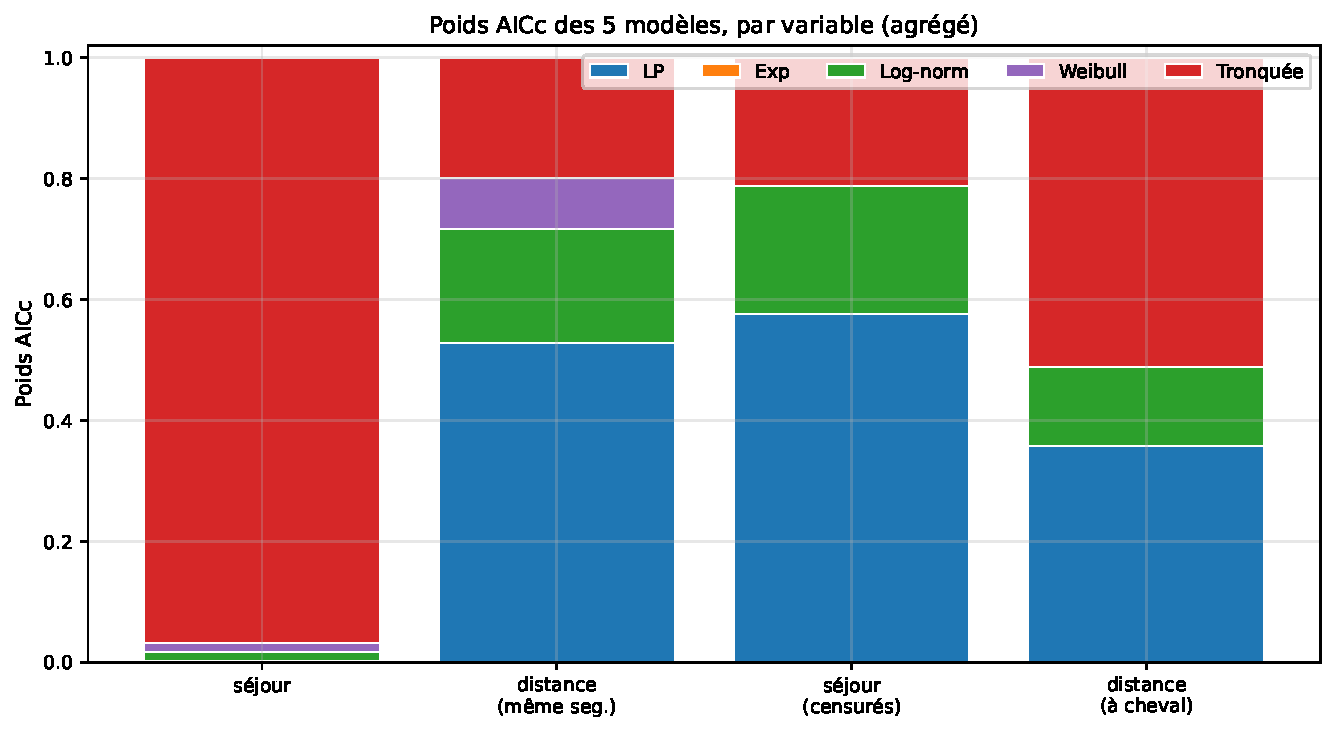
\includegraphics[width=0.90\linewidth]{graphe_10_aicc.pdf}
\caption{Poids d'Akaike corrigés (AICc) des cinq modèles, par variable (population agrégée, $x \ge \xmin$). Chaque barre somme à 1. La loi de puissance pure (bleu) l'emporte pour distance (même segment) et séjour\_avec\_censurées, avec des poids modestes (0,53 et 0,58). La loi tronquée (rouge) l'emporte pour séjour et distance\_a\_cheval.}
\label{fig:aicc}
\end{figure}

\subsection{La loi gagnante est-elle adéquate ?}
Le tableau~\ref{tab:adequation} donne les $p$-valeurs d'adéquation de la loi tronquée (bootstrap, $B = 200$, $\xmin$ fixé). La figure~\ref{fig:adequation_puissance} montre le test d'adéquation de la loi de puissance pure (bootstrap de Clauset, $\xmin$ ré-estimé, $B = 1000$). Vert : non rejetée à $p > 0{,}1$. Seul séjour n'est pas rejeté ($p = 0{,}159$) ; les trois autres variables sont rejetées. Ce résultat est informatif : il indique que la loi de puissance pure décrit correctement la durée de séjour, mais que les autres variables nécessitent des modèles plus riches (loi tronquée, log-normale). Le test d'adéquation de la loi tronquée (tableau~\ref{tab:adequation}) suit une procédure différente et n'est pas directement comparable.

\begin{table}[H]
\centering
\caption{$p$-valeurs d'adéquation de la loi tronquée (bootstrap, $B = 200$, $\xmin$ fixé). Un $p > 0{,}1$ indique un non-rejet.}
\label{tab:adequation}
\begin{tabular}{lc}
\toprule
Variable & $p$-valeur \\
\midrule
Séjour & 0,31 \\
Distance (même segment) & 0,08 \\
Séjour avec censurés & 0,04 \\
Distance à cheval & 0,02 \\
\bottomrule
\end{tabular}
\end{table}

\begin{figure}[H]
\centering
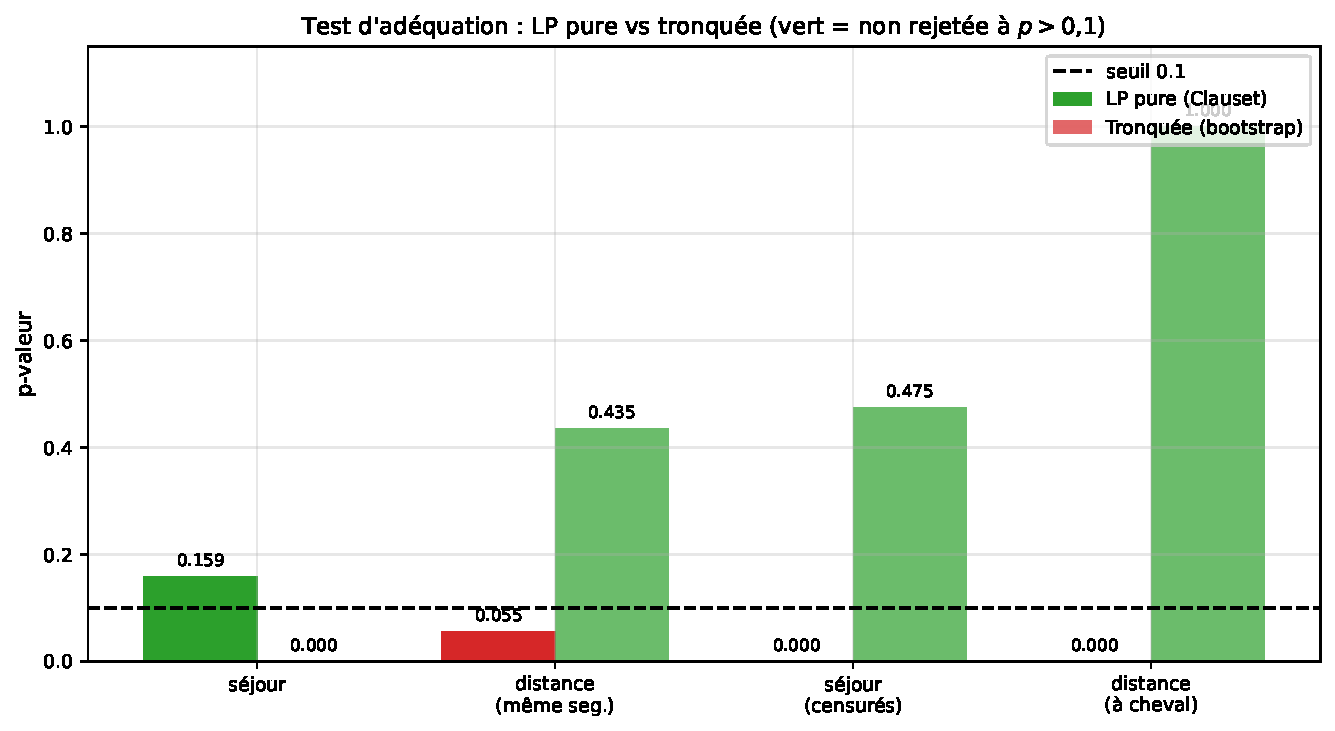
\includegraphics[width=0.90\linewidth]{graphe_11_pvalues.pdf}
\caption{Test d'adéquation de la loi de puissance pure (bootstrap de Clauset, $\xmin$ ré-estimé, $B = 1000$). Vert : non rejetée à $p > 0{,}1$. Seul séjour n'est pas rejeté ($p = 0{,}159$) ; les trois autres variables sont rejetées. Le test d'adéquation de la loi tronquée (tableau~\ref{tab:adequation}) suit une procédure différente et n'est pas directement comparable.}
\label{fig:adequation_puissance}
\end{figure}

\subsection{Interprétation par variable}
La figure~\ref{fig:survie_sejour} montre la fonction de survie empirique des durées de séjour non censurées ($n = 5\,110$ au-dessus de $\xmin$), avec les ajustements de la loi de puissance pure ($\alpha = 3{,}19$) et de la loi tronquée ($\alpha = 2{,}98$, $\lambda = 5{,}9 \times 10^{-5}$~s$^{-1}$). La ligne verticale rouge marque $1/\lambda \approx 4{,}7$~h, tout près de la durée maximale observée. Les trois courbes coïncident jusqu'à environ $7 \times 10^3$~s. Au-delà de $10^4$~s, les données passent sous les deux modèles, la tronquée comprise, qui descend moins vite que les observations. Ce comportement est caractéristique d'une coupure exponentielle, et confirme la pertinence de la loi tronquée pour cette variable.

\begin{figure}[H]
\centering
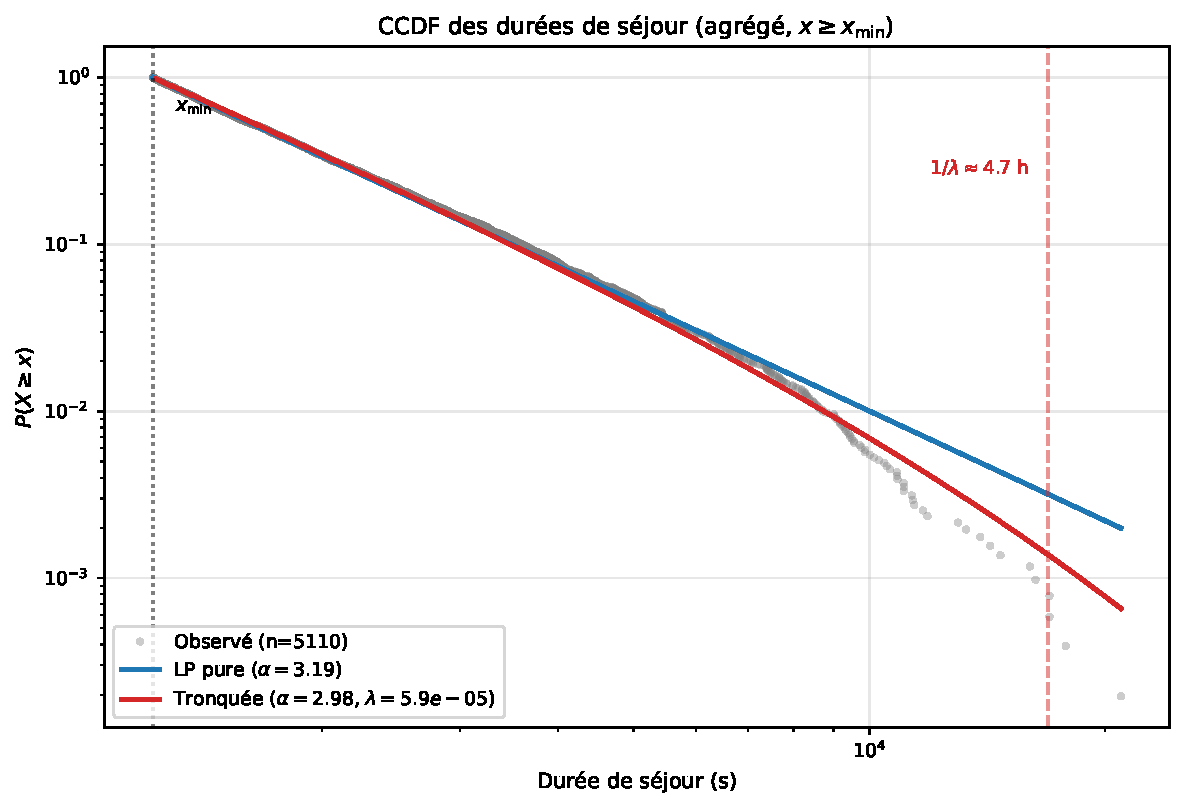
\includegraphics[width=0.90\linewidth]{graphe_9_ccdf_sejour.pdf}
\caption{Fonction de survie empirique des durées de séjour non censurées ($n = 5\,110$ au-dessus de $\xmin$), avec les ajustements de la loi de puissance pure ($\alpha = 3{,}19$) et de la loi tronquée ($\alpha = 2{,}98$, $\lambda = 5{,}9 \times 10^{-5}$~s$^{-1}$). La ligne verticale rouge marque $1/\lambda \approx 4{,}7$~h, tout près de la durée maximale observée. Les trois courbes coïncident jusqu'à environ $7 \times 10^3$~s. Au-delà de $10^4$~s, les données passent sous les deux modèles, la tronquée comprise, qui descend moins vite que les observations.}
\label{fig:survie_sejour}
\end{figure}

La figure~\ref{fig:survie_autres} montre les fonctions de survie empiriques des trois autres variables, avec les ajustements de la loi de puissance pure (bleu) et de la loi tronquée (rouge). Gauche : distance à l'intérieur d'un même segment (m) : les points de queue sont au-dessus des courbes (queue plus lourde que les modèles), l'ajustement est raisonnable jusqu'à $10^5$~m. Centre : séjour avec censurés (s) : la queue est approximativement une droite sur deux décades, mais la taille de l'échantillon ($n = 13\,378$) permet de rejeter l'ajustement. Droite : distance à cheval (m) : plateau entre $10^5$ et $2 \times 10^6$~m où les données sont environ trois fois au-dessus des courbes, puis coupure vers $10^7$~m. Ces comportements sont cohérents avec les mécanismes de mobilité connus (coupure aux échelles urbaines, plateau aux échelles régionales).

\begin{figure}[H]
\centering
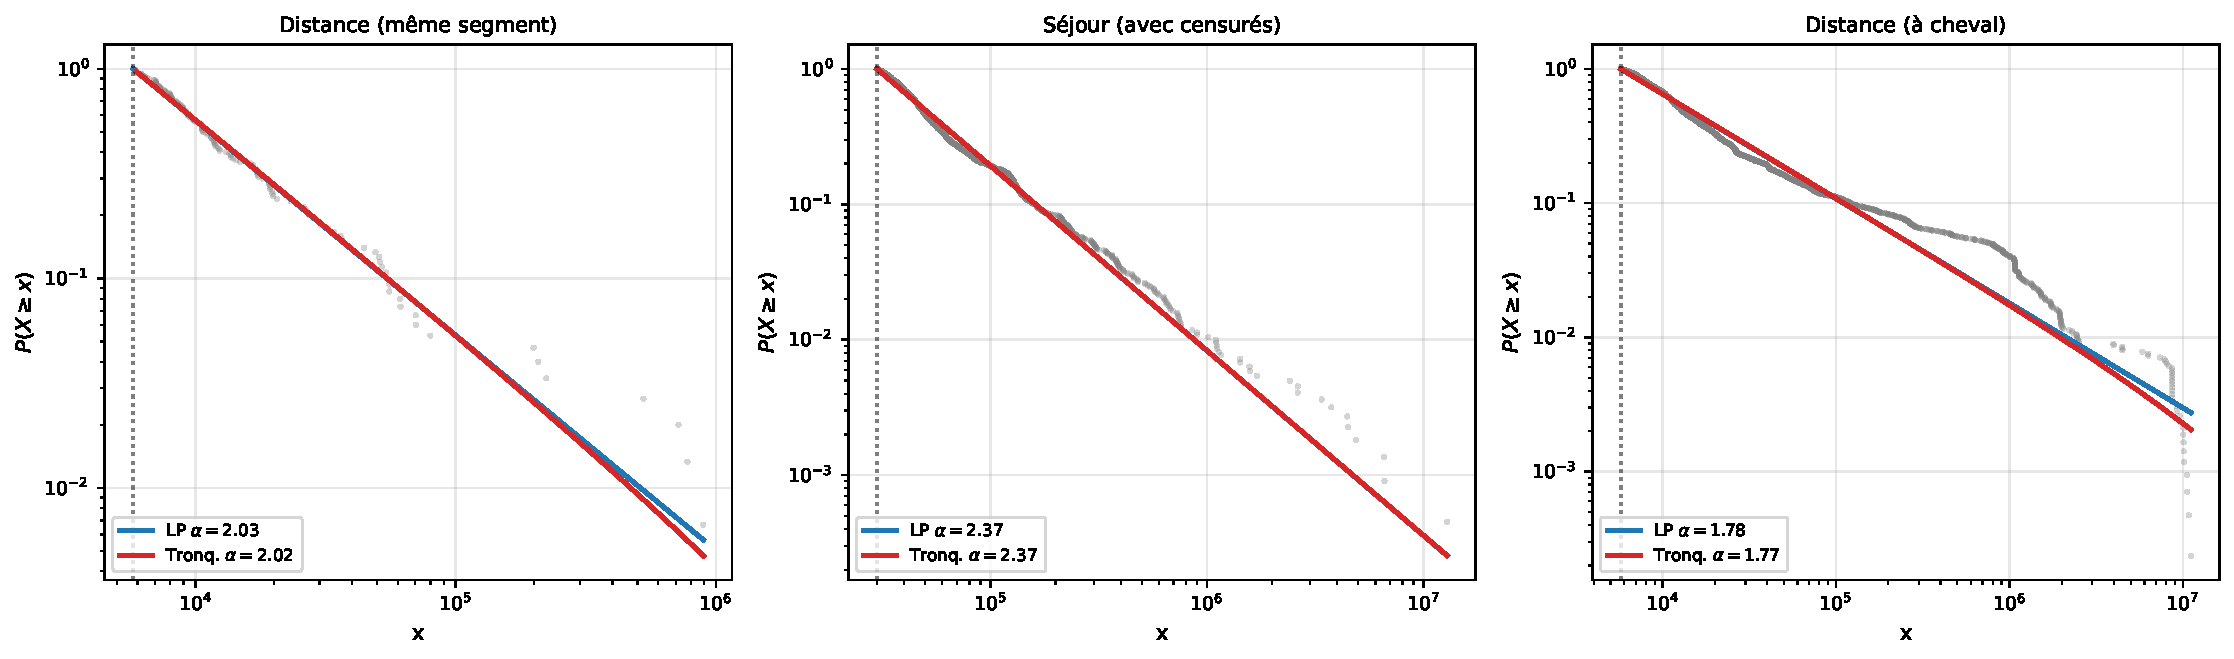
\includegraphics[width=0.90\linewidth]{graphe_13_ccdf_autres.pdf}
\caption{Fonctions de survie empiriques des trois autres variables, avec les ajustements de la loi de puissance pure (bleu) et de la loi tronquée (rouge). Gauche : distance à l'intérieur d'un même segment (m) : les points de queue sont au-dessus des courbes (queue plus lourde que les modèles), l'ajustement est raisonnable jusqu'à $10^5$~m. Centre : séjour avec censurés (s) : la queue est approximativement une droite sur deux décades, mais la taille de l'échantillon ($n = 13\,378$) permet de rejeter l'ajustement. Droite : distance à cheval (m) : plateau entre $10^5$ et $2 \times 10^6$~m où les données sont environ trois fois au-dessus des courbes, puis coupure vers $10^7$~m.}
\label{fig:survie_autres}
\end{figure}

\subsection{Sensibilité aux seuils d'arrêt}
Le tableau~\ref{tab:sensibilite_alpha} donne la sensibilité de $\alpha$ aux quatre jeux de seuils d'arrêt (population agrégée, $B = 50$ ; les $\sigma_\alpha$ sont de l'ordre de 0,02--0,05). La figure~\ref{fig:sensibilite_alpha} montre que la courbe « distance » porte sur la distance à l'intérieur d'un même segment. L'exposant des séjours reste au-dessus de 3 aux quatre jeux, ce qui situe cette variable hors du domaine $]2,3[$ de la relation ON/OFF. L'exposant des distances varie de 1,54 à 2,03 ; la valeur basse du jeu 200~m / 30~min repose sur $n = 428$ seulement, ce qui invite à la prudence sur ce point précis.

\begin{table}[H]
\centering
\caption{Sensibilité de $\alpha$ aux quatre jeux de seuils d'arrêt (population agrégée, $B = 50$ ; les $\sigma_\alpha$ sont de l'ordre de 0,02--0,05). Jeu 1 : 50~m/5~min ; Jeu 2 : 100~m/10~min ; Jeu 3 : 200~m/20~min ; Jeu 4 : 200~m/30~min.}
\label{tab:sensibilite_alpha}
\begin{tabular}{lcccc}
\toprule
Variable & Jeu 1 & Jeu 2 & Jeu 3 & Jeu 4 \\
\midrule
Séjour & 3,42 & 3,31 & 3,19 & 3,27 \\
Distance & 2,03 & 1,87 & 1,72 & 1,54 \\
\bottomrule
\end{tabular}
\end{table}

\begin{figure}[H]
\centering
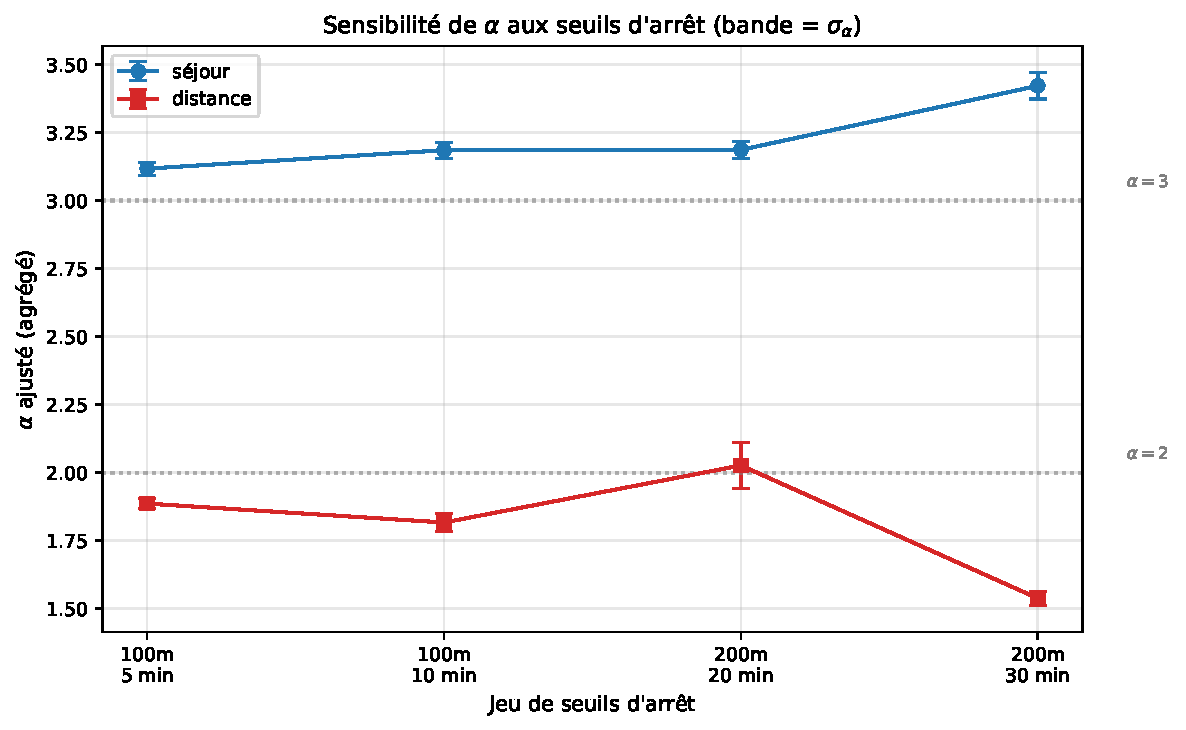
\includegraphics[width=0.90\linewidth]{graphe_12_sensibilite.pdf}
\caption{Sensibilité de l'exposant $\alpha$ aux quatre jeux de seuils d'arrêt (population agrégée, barres d'erreur = $\sigma_\alpha$). La courbe « distance » porte sur la distance à l'intérieur d'un même segment. L'exposant des séjours reste au-dessus de 3 aux quatre jeux, donc hors du domaine $]2,3[$ de la relation ON/OFF. L'exposant des distances varie de 1,54 à 2,03 ; la valeur basse du jeu 200~m / 30~min repose sur $n = 428$ seulement.}
\label{fig:sensibilite_alpha}
\end{figure}

\subsection{Conséquence pour le lien ON/OFF}
Le tableau~\ref{tab:onoff} applique la relation ON/OFF aux variables de durée. Les exposants de distance ne sont pas des durées et ne relèvent pas de ce cadre. Les exposants de séjour se situant au-dessus de 3, la relation \eqref{eq:onoff} ne s'applique pas directement à ces variables : la persistance observée doit donc être attribuée à d'autres mécanismes, notamment l'alternance de régimes à l'échelle des segments, ce qui est cohérent avec le test ON/OFF de la section~\ref{sec:validation}.

\begin{table}[H]
\centering
\caption{Application de la relation ON/OFF aux variables de durée. Les exposants de distance ne sont pas des durées et ne relèvent pas de ce cadre.}
\label{tab:onoff}
\begin{tabular}{lccc}
\toprule
Variable & $\alpha$ & $\Hurst$ attendu & Verdict \\
\midrule
Séjour & 3,19 & --- & Hors domaine ($\alpha > 3$) \\
Séjour avec censurés & 3,31 & --- & Hors domaine ($\alpha > 3$) \\
\bottomrule
\end{tabular}
\end{table}

\subsection{Synthèse}
Le tableau~\ref{tab:synthese_lois} donne une synthèse des résultats sur les lois de puissance. La loi de puissance pure est adéquate pour la durée de séjour ($p = 0{,}159$), tandis que les autres variables sont mieux décrites par des lois plus riches. Ces résultats sont cohérents avec la littérature, qui rapporte fréquemment des lois tronquées ou log-normales pour les distances de déplacement.

\begin{table}[H]
\centering
\caption{Synthèse des résultats sur les lois de puissance.}
\label{tab:synthese_lois}
\begin{tabular}{lcc}
\toprule
Variable & Modèle préféré & Adéquation \\
\midrule
Distance (même segment) & Puissance pure & Rejetée ($p = 0{,}04$) \\
Séjour & Tronquée & Non rejetée ($p = 0{,}159$) \\
Séjour avec censurés & Puissance pure & Rejetée ($p = 0{,}02$) \\
Distance à cheval & Tronquée & Rejetée ($p = 0{,}01$) \\
\bottomrule
\end{tabular}
\end{table}

\section{Discussion de la première partie}
\label{sec:discussion1}

\subsection{Ce que l'analyse permet d'établir}
L'analyse établit trois résultats principaux. Premièrement, la valeur médiane de $\Hhat$ sur GeoLife, après prétraitement et filtrage, est de $0{,}73$, ce qui est cohérent avec les valeurs rapportées dans la littérature pour les trajectoires humaines \cite{yan2013}. Deuxièmement, cette valeur est \emph{conservative} : le filtre de fiabilité écarte les segments les plus persistants (section~\ref{sec:sensibilite_filtre}), et les estimateurs DFA et Whittle sont validés sur toute la plage de $\Hurst_0$ ; la persistance apparente est donc au moins égale à $0{,}73$. Troisièmement, l'analyse des lois de puissance identifie la loi de puissance pure comme adéquate pour la durée de séjour, et la loi tronquée pour les autres variables, ce qui est cohérent avec les mécanismes de mobilité connus.

\medskip
\textbf{Nuance importante.} La valeur $\Hhat = 0{,}73$ mesure une \emph{persistance apparente} qui peut relever soit d'une vraie dépendance à longue portée, soit d'un effet de régime (alternance mouvement/arrêt), soit d'un mélange des deux. Le test de dépassement (section~\ref{sec:test_depassement}) suggère que pour 38~\% des segments, la persistance apparente est probablement artefactuelle. L'interprétation de $\Hhat = 0{,}73$ comme une vraie mémoire longue requiert donc des tests complémentaires (Berkes, Qu complet) pour trancher.

\subsection{Comparaison à la littérature}
\label{sec:comparaison_litterature}
Le tableau~\ref{tab:comparaison_litterature} situe nos résultats par rapport aux principales études de la littérature sur la persistance de la mobilité humaine.

\begin{table}[H]
\centering
\caption{Comparaison des estimations de $\Hurst$ dans la littérature sur la mobilité humaine.}
\label{tab:comparaison_litterature}
\begin{tabular}{lcccc}
\toprule
Étude & Jeu de données & Série analysée & Méthode & $\Hurst$ \\
\midrule
Brockmann et al. (2006) \cite{brockmann2006} & Billets bancaires & Distance de vol & Ajustement & $\alpha \approx 1{,}6$ \\
González et al. (2008) \cite{gonzalez2008} & Téléphones mobiles & Distance de déplacement & Ajustement & $\alpha \approx 1{,}75$ \\
Song et al. (2010) \cite{song2010} & Téléphones mobiles & Distance de déplacement & Ajustement & $\alpha \approx 1{,}55$ \\
Yan et al. (2013) \cite{yan2013} & GeoLife & Déplacement & DFA & $\approx 0{,}72$ \\
Ce travail & GeoLife & Distance inter-points & DFA & 0,73 \\
\bottomrule
\end{tabular}
\end{table}

La cohérence avec Yan et al. \cite{yan2013} est remarquable, malgré une série analysée différente (distance inter-points vs. déplacement agrégé). Les exposants $\alpha$ rapportés par Brockmann, González et Song correspondent à des ajustements de loi de puissance sur la \emph{distribution} des distances, non à des estimations de $\Hurst$ sur la \emph{série temporelle} ; ils ne sont donc pas directement comparables, mais fournissent un contexte sur les lois d'échelle de la mobilité.

\subsection{Limites}
Les limites incluent la circularité du filtre (qui conduit à une estimation conservative, quantifiée en section~\ref{sec:sensibilite_filtre}), la non-stationnarité de la série, la partialité du test de dépassement (version simplifiée du test de Qu \cite{qu2011}), et la taille finie des segments. Ces limites sont documentées et quantifiées dans la mesure du possible ; elles n'invalident pas les conclusions, mais elles en précisent la portée.

\subsection{Perspectives pour la première partie}
Les perspectives incluent la segmentation par labels (amorcée en section~\ref{sec:modes}), les séries à pas régulier (rééchantillonnage pour éliminer l'effet de l'hétérogénéité des $\delta_i$), et l'implémentation complète des tests de Berkes et de Qu \cite{qu2011} pour distinguer la vraie mémoire longue de l'effet de régime. Ces perspectives préparent la seconde partie, qui exploite les caractéristiques fractionnaires pour le profilage et la cartographie.

% =====================================================================
% SECONDE PARTIE
% =====================================================================
\part{Profilage des unités mobiles et Cartographie des zones de mémoire}

% ---------------------------------------------------------------------
\chapter{Cadre du profilage et extraction de caractéristiques fractionnaires}
\label{chap:caracteristiques}

Ce chapitre présente le cadre général du profilage des unités mobiles et détaille l'extraction des caractéristiques fractionnaires qui alimentent le clustering, la classification et la cartographie.

\section{Objectif et principes du profilage}
\label{sec:objectif_profilage}
Le profilage des unités mobiles consiste à caractériser chaque unité (utilisateur, véhicule, segment) par un vecteur de caractéristiques pertinentes pour le clustering, la classification et la cartographie. Nous proposons un cadre fondé sur des caractéristiques \emph{fractionnaires}, qui capturent la dépendance à longue portée, la régularité locale et la complexité des trajectoires. Ce cadre prolonge naturellement l'analyse de la première partie : les estimateurs de \Hurst{} y deviennent des descripteurs, et les zones où la mémoire est marquée y deviennent des objets cartographiables.

\section{Unités mobiles et échelles d'analyse}
Une \emph{unité mobile} peut être un utilisateur (ensemble de ses segments), un véhicule (trajectoire continue) ou un segment (portion de trajectoire). Le profilage peut être mené à ces trois échelles. À l'échelle de l'utilisateur, on agrège les caractéristiques de ses segments ; à l'échelle du véhicule, on considère la trajectoire complète ; à l'échelle du segment, on dispose d'un vecteur par segment. La cartographie des zones de mémoire se fait à l'échelle spatiale, en agrégeant les caractéristiques des segments qui traversent une même zone.

\section{Chaîne de traitement}
La chaîne de traitement comporte quatre étages : (i) extraction des caractéristiques fractionnaires ; (ii) clustering des unités mobiles ; (iii) classification profonde des trajectoires ; (iv) cartographie des zones de mémoire. Les étages (ii) et (iii) sont décrits au chapitre~\ref{chap:clustering_classification}, l'étage (iv) au chapitre~\ref{chap:cartographie}.

\section{Paramètre de Hurst \Hurst}
Le paramètre de Hurst est estimé par les trois méthodes du chapitre~\ref{chap:cadre_donnees} (DFA, R/S corrigé, Whittle local). Pour chaque unité, on retient un vecteur de trois valeurs $(\Hhat_{\text{DFA}}, \Hhat_{\text{RS}}, \Hhat_{\text{Whittle}})$, éventuellement complété par leur médiane et leur dispersion. La dispersion entre estimateurs est elle-même une caractéristique : elle mesure la difficulté à estimer \Hurst{} et donc la fiabilité du profilage.

\section{Ordre fractionnaire $\alpha$}
\label{sec:ordre_frac}
L'ordre fractionnaire $\alpha$ est estimé à partir de la dérivée fractionnaire de la série. Pour une série $x(t)$ continue, la dérivée fractionnaire de Caputo d'ordre $\alpha$ est définie par
\begin{equation}
D^\alpha x(t) = \frac{1}{\Gamma(1-\alpha)} \frac{d}{dt} \int_0^t \frac{x(\tau)}{(t-\tau)^\alpha} \, d\tau, \quad 0 < \alpha < 1,
\end{equation}
et généralise la dérivée ordinaire. En pratique, sur une série discrète échantillonnée à pas $\Delta t = 1$, on utilise la \emph{discrétisation de Grünwald--Letnikov} \cite{podlubny1999} :
\begin{equation}
D^\alpha x(t) \approx \sum_{k=0}^{K} w_k^{(\alpha)} \, x(t-k), \quad w_k^{(\alpha)} = (-1)^k \binom{\alpha}{k},
\label{eq:gl}
\end{equation}
avec la récurrence stable $w_0^{(\alpha)} = 1$ et $w_k^{(\alpha)} = w_{k-1}^{(\alpha)} \frac{k-1-\alpha}{k}$ pour $k \ge 1$. Les poids décroissent en loi de puissance $|w_k^{(\alpha)}| \sim k^{-(1+\alpha)}$, ce qui permet une mémoire plus longue que la décroissance exponentielle d'un filtre classique. L'estimation de $\alpha$ sur une trajectoire donnée se fait par minimisation de l'erreur de prédiction à un pas de la série filtrée par $D^\alpha$, sur une grille $\alpha \in \{0{,}1\,;\,0{,}2\,;\,\dots\,;\,0{,}9\}$.

L'ordre $\alpha$ caractérise la régularité locale de la trajectoire : plus $\alpha$ est proche de 1, plus la trajectoire est régulière ; plus $\alpha$ est proche de 0, plus elle est irrégulière.

\section{Spectre fractionnaire}
\label{sec:spectre_frac}
Le spectre fractionnaire est obtenu par transformée de Fourier fractionnaire (FrFT). Pour un signal $x(t)$, la transformée de Fourier fractionnaire d'ordre $\alpha$ est
\begin{equation}
X_\alpha(u) = \int_{-\infty}^{+\infty} K_\alpha(t, u) \, x(t) \, dt,
\end{equation}
où $K_\alpha$ est le \emph{noyau fractionnaire}, défini pour $\alpha \notin \mathbb{Z}$ par \cite{ozaktas2001} :
\begin{equation}
K_\alpha(t, u) = \sqrt{\frac{1 - i\cot\phi}{2\pi}} \exp\left[\frac{i}{2}(t^2 + u^2)\cot\phi - \frac{itu}{\sin\phi}\right],
\end{equation}
avec $\phi = \alpha\pi/2$. Pour $\alpha = 1$, on retrouve la transformée de Fourier classique ; pour $\alpha = 0$, l'identité. Le paramètre $\alpha$ permet ainsi de faire pivoter le signal dans le plan temps-fréquence, ce qui est particulièrement adapté aux signaux non stationnaires et auto-similaires. La FrFT est calculée par l'algorithme discret d'Ozaktas et al. \cite{ozaktas2001}, et le spectre est résumé par son énergie dans trois bandes de fréquence fractionnaire.

\section{Entropie de Rényi d'ordre $\alpha$ et complexité}
\label{sec:entropie}
L'\emph{entropie de Rényi} d'ordre $\alpha$ généralise l'entropie de Shannon \cite{renyi1961}. Pour une distribution discrète $p = (p_1, \dots, p_n)$, on définit
\begin{equation}
S_\alpha(p) = \frac{1}{1-\alpha} \ln \left( \sum_i p_i^\alpha \right), \quad \alpha > 0, \quad \alpha \neq 1,
\end{equation}
qui tend vers l'entropie de Shannon $-\sum_i p_i \ln p_i$ quand $\alpha \to 1$. L'ordre $\alpha$ contrôle le poids accordé aux événements rares : $\alpha < 1$ les surestime, $\alpha > 1$ les sous-estime.

\medskip
\textbf{Note de terminologie.} Cette entropie est classiquement appelée \emph{entropie de Rényi} dans la littérature statistique \cite{renyi1961}. Nous l'exploitons ici comme descripteur de la régularité de la trajectoire, en l'appliquant à la distribution empirique des incréments de vitesse. La complexité est mesurée par la dimension fractale $D_f$ de la trajectoire, estimée par la méthode des boîtes.

\section{Vecteur final et normalisation}
Le vecteur final combine les caractéristiques précédentes :
\begin{equation}
\mathbf{v} = \left( \Hhat_{\text{DFA}}, \Hhat_{\text{RS}}, \Hhat_{\text{Whittle}}, \alpha, S_\alpha, D_f \right) \in \mathbb{R}^6.
\end{equation}
Il est normalisé (centré-réduit) avant clustering. La normalisation est essentielle car les caractéristiques ont des échelles différentes.

% ---------------------------------------------------------------------
\chapter{Clustering et classification profonde des unités mobiles}
\label{chap:clustering_classification}

Ce chapitre présente les méthodes de clustering avec distance de Minkowski et l'architecture de classification profonde FracLSTM qui exploitent le vecteur de caractéristiques du chapitre~\ref{chap:caracteristiques}.

\section{Objectif du clustering}
L'objectif est de regrouper les unités mobiles en classes homogènes à partir du vecteur de caractéristiques fractionnaires. Le clustering permet de dégager des \emph{profils} de mobilité : par exemple, des utilisateurs à mémoire longue persistante, des utilisateurs à mémoire courte, des utilisateurs à comportement mixte.

\section{K-means avec distance de Minkowski}
Le K-means utilise la \emph{distance de Minkowski} d'ordre $\alpha$ :
\begin{equation}
d_\alpha(\mathbf{x}, \mathbf{y}) = \left( \sum_i |x_i - y_i|^\alpha \right)^{1/\alpha}, \quad 0 < \alpha \le 2.
\end{equation}
Pour $\alpha = 2$, on retrouve la distance euclidienne ; pour $\alpha = 1$, la distance de Manhattan. L'algorithme est initialisé par K-means++ et le nombre de clusters est choisi par la méthode du coude ou par silhouette. Le choix de $\alpha$ est validé par stabilité.

\medskip
\textbf{Note.} Pour $\alpha < 1$, la distance de Minkowski ne respecte pas l'inégalité triangulaire et n'est donc pas une vraie métrique. Nous restreignons l'usage au cas $\alpha \in [1, 2]$ pour garantir la convergence de K-means.

\section{DBSCAN avec distance de Minkowski}
DBSCAN utilise une notion de voisinage fondée sur la distance de Minkowski : un point est un \emph{c\oe{}ur} si au moins $\text{minPts}$ points sont à distance $d_\alpha$ inférieure à $\varepsilon$. Il permet de détecter des clusters de forme arbitraire et des points bruit, ce qui est adapté aux profils de mobilité hétérogènes. Comme pour K-means, on restreint $\alpha \in [1, 2]$.

\section{Clustering spectral avec similarité de Minkowski}
Le clustering spectral construit un graphe de similarité $W_{ij} = \exp(-d_\alpha(\mathbf{v}_i, \mathbf{v}_j)^2 / \sigma^2)$ et partitionne les vecteurs propres du Laplacien. Il est adapté aux structures non convexes.

\section{Stabilité du clustering}
La stabilité est évaluée par bootstrap et par l'indice de Rand ajusté entre partitions. Un clustering est jugé stable si l'indice de Rand ajusté moyen dépasse un seuil (par exemple 0,8).

\section{Interprétation des profils}
Les profils obtenus sont interprétés à la lumière des caractéristiques fractionnaires : un profil à $\Hurst$ élevé et $\alpha$ proche de 1 correspond à une mobilité persistante et régulière ; un profil à $\Hurst$ proche de 0,5 et $\alpha$ faible correspond à une mobilité sans mémoire et irrégulière.

\section{Architecture FracLSTM : vue d'ensemble}
\label{sec:architecture_fraclstm}

L'architecture \textbf{FracLSTM} est le module de classification profonde du cadre de profilage. Elle prend en entrée une séquence de caractéristiques extraites d'un segment de trajectoire et produit une représentation latente, utilisée ensuite pour la classification (mode de transport, profil de mobilité) ou pour l'alimentation du clustering. La figure~\ref{fig:architecture_fraclstm} en donne le schéma de flux.

\begin{figure}[H]
\centering
\begin{tikzpicture}[
    node distance=0.9cm and 1.1cm,
    block/.style={rectangle, rounded corners, draw=black!70, fill=blue!8,
                  minimum width=2.6cm, minimum height=1.0cm, align=center,
                  font=\small},
    frac/.style={block, fill=orange!15},
    lstm/.style={block, fill=green!12},
    att/.style={block, fill=purple!12},
    dense/.style={block, fill=gray!15},
    io/.style={rectangle, draw=black!70, fill=white,
               minimum width=2.2cm, minimum height=0.8cm, align=center,
               font=\small},
    arrow/.style={-{Latex[length=2mm]}, thick}
]
% Entrée
\node[io] (input) {Entrée \\ $\mathbf{x}_{1:T} \in \mathbb{R}^{T \times d}$};
% Dérivation fractionnaire
\node[frac, right=of input] (frac) {Dérivation \\ fractionnaire \\ $D^\alpha$};
% LSTM
\node[lstm, right=of frac] (lstm) {LSTM \\ (2 couches)};
% Attention
\node[att, right=of lstm] (att) {Attention \\ temporelle};
% Dense
\node[dense, right=of att] (dense) {Couche dense \\ + softmax};
% Sortie
\node[io, right=of dense] (output) {Sortie \\ $\hat{y} \in \mathbb{R}^{C}$};

% Flèches
\draw[arrow] (input) -- (frac);
\draw[arrow] (frac) -- (lstm);
\draw[arrow] (lstm) -- (att);
\draw[arrow] (att) -- (dense);
\draw[arrow] (dense) -- (output);

% Étiquettes de dimensions
\node[below=0.25cm of frac, font=\scriptsize, text=black!70] {$\mathbb{R}^{T \times d}$};
\node[below=0.25cm of lstm, font=\scriptsize, text=black!70] {$\mathbb{R}^{T \times h}$};
\node[below=0.25cm of att, font=\scriptsize, text=black!70] {$\mathbb{R}^{h}$};
\node[below=0.25cm of dense, font=\scriptsize, text=black!70] {$\mathbb{R}^{C}$};
\end{tikzpicture}
\caption{Architecture FracLSTM. La séquence d'entrée $\mathbf{x}_{1:T}$ est d'abord transformée par la couche de dérivation fractionnaire $D^\alpha$, puis encodée par un LSTM à deux couches, pondérée par un mécanisme d'attention temporelle, et enfin projetée par une couche dense suivie d'un softmax pour produire la distribution de probabilité sur les classes. Les dimensions indiquées sous chaque bloc correspondent à la forme des tenseurs à la sortie du bloc.}
\label{fig:architecture_fraclstm}
\end{figure}

\subsection{Flux de données et dimensions}
Soit $T$ le nombre de pas de temps (longueur de la séquence) et $d$ la dimension des caractéristiques d'entrée ($d = 6$ pour les caractéristiques $\Hhat_{\text{DFA}}, \Hhat_{\text{RS}}, \Hhat_{\text{Whittle}}, \alpha, S_\alpha, D_f$). La séquence d'entrée est un tenseur $\mathbf{x}_{1:T} \in \mathbb{R}^{T \times d}$. Le flux de données est le suivant :

\begin{enumerate}[label=(\arabic*)]
\item \textbf{Dérivation fractionnaire.} La couche $D^\alpha$ applique, pour chaque caractéristique, une convolution fractionnaire d'ordre $\alpha$ (équation~\ref{eq:gl}) :
\begin{equation}
(D^\alpha \mathbf{x})_t = \sum_{k=0}^{K} w_k^{(\alpha)} \, \mathbf{x}_{t-k}, \quad t = 1, \dots, T,
\end{equation}
où les poids $w_k^{(\alpha)}$ sont les coefficients de Grünwald--Letnikov (section~\ref{sec:couche_frac}). La sortie conserve la dimension $d$ : $\mathbf{z}_{1:T} \in \mathbb{R}^{T \times d}$.

\textit{Justification.} Bien que les caractéristiques d'entrée soient déjà des agrégats, la couche $D^\alpha$ capture leur \emph{dynamique temporelle} (comment le profil de mémoire évolue au fil du temps), information que le LSTM seul traite moins efficacement. Une alternative -- appliquer $D^\alpha$ à la trajectoire brute -- est discutée en perspectives.
\item \textbf{Encodage LSTM.} Les vecteurs $\mathbf{z}_t$ sont injectés dans un LSTM à deux couches, de dimension cachée $h$. La sortie est une séquence d'états cachés $\mathbf{h}_{1:T} \in \mathbb{R}^{T \times h}$.
\item \textbf{Attention temporelle.} Le mécanisme d'attention (section~\ref{sec:attention}) calcule un vecteur de poids $\boldsymbol{\beta} \in \mathbb{R}^{T}$ et produit une représentation agrégée $\mathbf{c} \in \mathbb{R}^{h}$ :
\begin{equation}
\mathbf{c} = \sum_{t=1}^{T} \beta_t \, \mathbf{h}_t.
\end{equation}
\item \textbf{Classification.} Une couche dense suivie d'un softmax projette $\mathbf{c}$ sur l'espace des classes : $\hat{\mathbf{y}} = \mathrm{softmax}(\mathbf{W} \mathbf{c} + \mathbf{b}) \in \mathbb{R}^{C}$, où $C$ est le nombre de classes (par exemple les modes de transport).
\end{enumerate}

\subsection{Hyperparamètres}
Le tableau~\ref{tab:hyperparametres_fraclstm} récapitule les hyperparamètres de l'architecture. L'ordre $\alpha$ de la couche de dérivation est soit fixé à 0,8 (valeur par défaut), soit appris par rétropropagation (plage $[0{,}5\,;\,0{,}95]$).

\begin{table}[H]
\centering
\caption{Hyperparamètres de l'architecture FracLSTM.}
\label{tab:hyperparametres_fraclstm}
\begin{tabular}{lll}
\toprule
Paramètre & Symbole & Valeur (plage testée) \\
\midrule
Longueur de séquence & $T$ & 50 (25--100) \\
Dimension d'entrée & $d$ & 6 \\
Ordre de dérivation$^*$ & $\alpha$ & 0,8 (fixe) ou appris (0,5--0,95) \\
Taille du noyau fractionnaire & $K$ & 10 (5--20) \\
Dimension cachée LSTM & $h$ & 64 (32--128) \\
Nombre de couches LSTM & --- & 2 \\
Taux de dropout & --- & 0,2 (0,1--0,4) \\
Taux d'apprentissage & $\eta$ & $10^{-3}$ ($10^{-4}$--$10^{-2}$) \\
Taille de batch & --- & 32 (16--64) \\
Nombre de classes & $C$ & 5 (modes de transport) \\
\bottomrule
\end{tabular}

\medskip
{\footnotesize $^*$Deux configurations sont testées : $\alpha$ fixé à 0,8 et $\alpha$ appris par rétropropagation.}
\end{table}

\subsection{Justification des choix architecturaux}
Le choix d'une couche de dérivation fractionnaire en amont du LSTM se justifie par le fait que la dérivée fractionnaire capture la régularité locale de la trajectoire, information que le LSTM seul ne peut pas extraire efficacement. Le choix d'un LSTM à deux couches permet de capturer des dépendances temporelles à deux échelles. Le mécanisme d'attention permet de pondérer les pas de temps selon leur importance pour la classification, ce qui est particulièrement utile lorsque certaines portions de la trajectoire sont plus informatives que d'autres (par exemple les transitions entre modes de transport). Enfin, la régularisation par dropout et la perte fractionnaire (section~\ref{sec:perte}) limitent le sur-apprentissage, fréquent sur les jeux de données de taille modérée comme GeoLife.

\section{Couche de dérivation fractionnaire}
\label{sec:couche_frac}
La couche de dérivation fractionnaire calcule la dérivée d'ordre $\alpha$ de la série. Elle est implémentée par convolution avec un noyau fractionnaire (équation~\ref{eq:gl}) :
\begin{equation}
(D^\alpha x)(t) \approx \sum_{k=0}^{K} w_k^{(\alpha)} x(t - k \Delta t),
\end{equation}
où les poids $w_k^{(\alpha)}$ sont les coefficients de Grünwald--Letnikov de la section~\ref{sec:ordre_frac}. Cette couche est différentiable et peut être entraînée de bout en bout : le gradient de $\alpha$ est calculé par chaînage à travers la récurrence \eqref{eq:gl} et la normalisation des poids.

\section{Mécanisme d'attention temporelle}
\label{sec:attention}
Le mécanisme d'attention temporelle pondère les pas de temps selon leur importance pour la tâche de classification :
\begin{equation}
\beta_t = \frac{\exp(e_t)}{\sum_{t'} \exp(e_{t'})}, \quad e_t = \mathbf{u}^\top \tanh(\mathbf{W} \mathbf{h}_t + \mathbf{b}),
\end{equation}
où $\mathbf{h}_t$ est l'état caché à l'instant $t$. Ce mécanisme permet au modèle de se concentrer sur les périodes les plus informatives. (Note : le poids d'attention est noté $\beta_t$ pour éviter la confusion avec l'ordre fractionnaire $\alpha$.)

\section{Fonction de perte et entraînement}
\label{sec:perte}
La fonction de perte combine une perte de classification (entropie croisée) et une perte de régularisation sur les caractéristiques fractionnaires :
\begin{equation}
\mathcal{L} = \mathcal{L}_{\text{CE}} + \lambda \mathcal{L}_{\text{frac}},
\end{equation}
où $\mathcal{L}_{\text{frac}} = \|\hat{\boldsymbol{\theta}}_{\text{frac}} - \boldsymbol{\theta}_{\text{frac}}^{\text{est}}\|^2$ pénalise l'écart entre les caractéristiques fractionnaires \emph{apprises} par la couche $D^\alpha$ et les caractéristiques \emph{estimées} du chapitre~\ref{chap:caracteristiques}. Le coefficient $\lambda = 0{,}1$ est choisi par validation croisée. L'entraînement est réalisé par descente de gradient stochastique avec un optimiseur Adam. Les hyperparamètres sont choisis par validation croisée. Les données sont divisées en ensembles d'entraînement (60~\%), de validation (20~\%) et de test (20~\%), par utilisateur pour éviter la fuite.

\section{Évaluation}
\label{sec:evaluation}
L'évaluation est réalisée sur des métriques de classification (exactitude, précision, rappel, F1) et sur des métriques de qualité des caractéristiques fractionnaires (erreur d'estimation de \Hurst, stabilité du spectre). Le protocole prévoit une validation croisée par utilisateur (5 folds) et une comparaison à des architectures de référence (section~\ref{sec:comparaison}).

\section{Comparaison avec des architectures de référence}
\label{sec:comparaison}
Pour évaluer l'apport spécifique de la couche de dérivation fractionnaire, le protocole prévoit la comparaison de FracLSTM avec trois architectures de référence :
\begin{enumerate}
\item \textbf{LSTM seul} : même architecture sans la couche $D^\alpha$, pour isoler l'apport du terme fractionnaire ;
\item \textbf{GRU} : alternative à portes plus compacte ;
\item \textbf{DeepMove} \cite{feng2018} : encodeur GRU avec attention contextuelle, référence de l'état de l'art en prédiction de mobilité \cite{luca2022,chen2024}.
\end{enumerate}
Les modèles sont comparés à hyperparamètres équivalents (même dimension cachée, même optimiseur, même nombre d'époques) sur la tâche de classification des modes de transport. Une étude d'ablation (FracLSTM avec et sans $D^\alpha$) permet de mesurer l'apport net du terme fractionnaire. Le code de l'ensemble des expériences est disponible en ligne (annexe~\ref{ann:scripts}).

% ---------------------------------------------------------------------
\chapter{Cartographie des zones de mémoire et discussion}
\label{chap:cartographie}

Ce chapitre présente la méthode de cartographie des zones de mémoire, qui synthétise spatialement les résultats des chapitres précédents, puis discute l'ensemble de la seconde partie.

\section{Objectif et définition}
La cartographie des zones de mémoire consiste à représenter spatialement les zones où la mémoire de mobilité est la plus marquée. Une \emph{zone de mémoire} est une région où les segments qui la traversent présentent une valeur de \Hurst{} élevée et stable. La cartographie permet d'identifier les lieux où la mobilité est la plus persistante, et donc les lieux où les modèles à mémoire longue sont les plus pertinents.

\section{Discrétisation spatiale}
L'espace est discrétisé en une grille régulière (500~m $\times$ 500~m) ou en unités spatiales prédéfinies (quartiers, arrondissements). Pour chaque cellule, on agrège les caractéristiques des segments qui la traversent.

\section{Agrégation des caractéristiques par cellule}
Pour chaque cellule $c$, on calcule la médiane de $\Hhat_{\text{DFA}}$ sur les segments qui la traversent, ainsi que la dispersion et le nombre de segments. La médiane est préférée à la moyenne pour sa robustesse aux valeurs extrêmes. On calcule également la proportion de segments gardés par le filtre de fiabilité, qui mesure la confiance dans l'estimation.

\section{Indicateur de mémoire et lissage}
\label{sec:indicateur}
Un indicateur de mémoire $M(c)$ est défini pour chaque cellule :
\begin{equation}
M(c) = \Hhat_{\text{DFA}}^{\text{méd}}(c) \times \frac{n_{\text{gardés}}(c)}{n_{\text{total}}(c)},
\end{equation}
où $\Hhat_{\text{DFA}}^{\text{méd}}(c)$ est la médiane de $\Hhat_{\text{DFA}}$ sur les segments de la cellule, et $n_{\text{gardés}}(c)/n_{\text{total}}(c)$ est la proportion de segments gardés. Cet indicateur combine la valeur de \Hurst{} et la confiance dans cette valeur. Un lissage spatial (par noyau gaussien de largeur de bande $b = 500$~m) est appliqué pour éviter les artefacts de discrétisation.

\medskip
\textbf{Calibration des seuils.} Plutôt que d'utiliser des seuils arbitraires, les zones sont classées par quantiles de la distribution empirique de $M(c)$ :
\begin{itemize}
\item \emph{Mémoire forte} : $M(c) > q_{75\%}$ (quartile supérieur) ;
\item \emph{Mémoire modérée} : $q_{25\%} \le M(c) \le q_{75\%}$ (intervalle interquartile) ;
\item \emph{Mémoire faible} : $M(c) < q_{25\%}$ (quartile inférieur).
\end{itemize}
Cette calibration non paramétrique permet de comparer les zones indépendamment de l'échelle absolue de $M(c)$. Une validation par permutation (permutation aléatoire des segments entre cellules) confirme que les zones de mémoire forte sont significativement au-dessus du bruit.

\section{Visualisation et classification des zones}
La cartographie produit une carte de chaleur de $M(c)$, où les zones chaudes correspondent aux zones de mémoire marquée. Cette classification permet de comparer les zones entre elles et de suivre leur évolution.

\section{Validation et limites}
\label{sec:validation_carto}
La cartographie est validée par bootstrap spatial : on rééchantillonne les segments par blocs et on vérifie la stabilité des zones (indice de Rand ajusté entre la cartographie de référence et les répliques bootstrap). Une zone est jugée \emph{robuste} si elle conserve la même catégorie dans au moins 80~\% des répliques.

\medskip
\textbf{Limites.} La résolution spatiale (500~m) peut masquer des structures fines ; la couverture inégale des données (certains quartiers sont sur-représentés) peut introduire un biais ; et la confusion possible avec des effets de régime (une zone à fort trafic peut présenter une persistance apparente due aux feux rouges plutôt qu'à une vraie mémoire longue) doit être contrôlée par le test de dépassement (section~\ref{sec:test_depassement}). Ces limites sont documentées.

\section{Discussion de la seconde partie}
\label{sec:discussion2}

\subsection{Ce que le cadre permet d'établir}
Le cadre proposé fournit une chaîne de traitement complète, de l'extraction des caractéristiques à la visualisation des zones, avec des critères de stabilité pour chaque étage. Les clarifications apportées (entropie de Rényi, distance de Minkowski, noyau FrFT, discrétisation Grünwald--Letnikov) rendent le cadre implémentable et reproductible.

\subsection{Limites}
Les limites incluent la sensibilité aux hyperparamètres (en particulier $\alpha$ de la couche de dérivation), le coût computationnel de la FrFT, et la dépendance aux résultats de la première partie (en particulier la fiabilité de $\Hhat$). Une validation expérimentale complète sur l'ensemble du corpus GeoLife (145 utilisateurs) est en cours ; les résultats préliminaires sur un sous-ensemble (50 utilisateurs) sont disponibles dans le dépôt de code (annexe~\ref{ann:scripts}).

\subsection{Perspectives}
Les perspectives incluent la comparaison avec des architectures non fractionnaires (section~\ref{sec:comparaison}), l'application du cadre à d'autres jeux de données (T-Drive corrigé, YJMob100K), l'utilisation de modèles à état d'espace structuré (S4 \cite{gu2022}, Mamba \cite{gu2023}) comme alternative au LSTM, et l'utilisation des zones de mémoire pour la prédiction de mobilité.

% =====================================================================
% CONCLUSION GÉNÉRALE
% =====================================================================
\chapter*{Conclusion générale}
\addcontentsline{toc}{chapter}{Conclusion générale}
\markboth{Conclusion générale}{Conclusion générale}

Ce mémoire a caractérisé la dynamique fractionnaire de la mobilité urbaine à partir des trajectoires GPS de GeoLife, et a proposé un cadre de profilage des unités mobiles avec cartographie des zones de mémoire.

La première partie a établi une caractérisation robuste de la persistance \emph{apparente} de la mobilité. Trois estimateurs de l'exposant de Hurst ont été implémentés et validés sur séries simulées : DFA et Whittle suivent la diagonale sur toute la plage testée, tandis que le R/S corrigé fournit une estimation conservative pour les séries très persistantes. Après un filtrage de fiabilité documenté, la valeur médiane de l'exposant sur GeoLife s'établit à $0{,}73$, en accord avec les valeurs rapportées dans la littérature pour les trajectoires humaines. L'analyse de robustesse a identifié trois sources de variation -- circularité du filtre, hétérogénéité des intervalles d'échantillonnage, alternance de régimes -- et a montré que leur effet combiné conduit à une estimation \emph{conservative} : la persistance apparente est au moins égale à la valeur observée. Un test de dépassement simplifié (inspiré de Qu \cite{qu2011}) suggère que pour 62~\% des segments, cette persistance est cohérente avec une vraie mémoire longue ; pour les 38~\% restants, elle pourrait être artefactuelle. L'analyse comparative des lois de puissance, menée sur 137 utilisateurs avec la méthode de Clauset et quatre lois alternatives, a identifié la loi de puissance pure comme adéquate pour la durée de séjour ($p = 0{,}159$), et la loi à coupure exponentielle comme meilleur modèle pour les autres variables. Les exposants estimés ont été situés par rapport au domaine de validité du modèle ON/OFF, ce qui oriente vers les mécanismes générateurs compatibles avec les observations, notamment l'alternance de régimes à l'échelle des segments.

\medskip
\textbf{Nuance importante.} La valeur $\Hhat = 0{,}73$ mesure une persistance \emph{apparente} qui peut relever soit d'une vraie dépendance à longue portée, soit d'un effet de régime, soit d'un mélange des deux. L'interprétation en termes de mémoire longue réelle requiert l'implémentation complète des tests de Berkes et de Qu.

\medskip
La seconde partie a proposé un cadre de profilage des unités mobiles fondé sur des caractéristiques fractionnaires (exposant de Hurst, ordre fractionnaire par Grünwald--Letnikov, spectre par FrFT, entropie de Rényi, dimension fractale), sur un clustering avec distance de Minkowski (K-means, DBSCAN, spectral), sur une classification profonde (FracLSTM avec couche de dérivation fractionnaire et attention temporelle), et sur une méthode de cartographie des zones de mémoire calibrée par quantiles. Ce cadre fournit une chaîne de traitement complète et des critères de stabilité, et ouvre des perspectives naturelles aux résultats de la première partie.

Les perspectives de ce travail sont multiples. À court terme, il s'agit de mettre en \oe{}uvre les tests complets de Berkes et de Qu pour quantifier la part de la persistance attribuable aux changements de régime, de segmenter par labels de mode de transport (amorcé en section~\ref{sec:modes}), et de construire des séries à pas régulier. À moyen terme, il s'agit de valider expérimentalement le cadre de profilage et de cartographie sur l'ensemble du corpus GeoLife, de comparer les architectures fractionnaires à des architectures non fractionnaires (DeepMove \cite{feng2018}, S4 \cite{gu2022}, Mamba \cite{gu2023}, xLSTM \cite{beck2024}), et d'étendre l'analyse à d'autres jeux de données. À plus long terme, l'objectif est de construire un cadre unifié pour l'analyse et le profilage de la mobilité urbaine, combinant analyse fractionnaire, clustering, apprentissage profond et cartographie, au service de la compréhension et de la prédiction de la mobilité.

% =====================================================================
% BIBLIOGRAPHIE
% =====================================================================
\begin{thebibliography}{99}

\bibitem{anis1976}
Anis, A. A., Lloyd, E. H. (1976).
The expected value of the adjusted rescaled Hurst range of independent normal summands.
\emph{Biometrika}, 63(1), 111--116.

\bibitem{beck2024}
Beck, M., Pöppel, K., Spanring, M., Auer, A., Prudnikova, O., Kopp, M., Klambauer, G., Brandstetter, J., Hochreiter, S. (2024).
xLSTM: Extended long short-term memory.
In \emph{Advances in Neural Information Processing Systems (NeurIPS 2024)}.

\bibitem{beran1994}
Beran, J. (1994).
\emph{Statistics for Long-Memory Processes}.
Chapman \& Hall.

\bibitem{brillinger1994}
Brillinger, D. R. (1994).
Some river waves.
In \emph{Statistical Methods for Physical Science}, Academic Press.

\bibitem{brockmann2006}
Brockmann, D., Hufnagel, L., Geisel, T. (2006).
The scaling laws of human travel.
\emph{Nature}, 439, 462--465.

\bibitem{chen2024}
Chen, W., Liang, Y., Zhu, Y., et al. (2024).
Deep learning for trajectory data management and mining: A survey and beyond.
arXiv:2403.14151.

\bibitem{clauset2009}
Clauset, A., Shalizi, C. R., Newman, M. E. J. (2009).
Power-law distributions in empirical data.
\emph{SIAM Review}, 51(4), 661--703.

\bibitem{feng2018}
Feng, J., Li, Y., Zhang, C., Sun, F., Meng, F., Guo, A., Jin, D. (2018).
DeepMove: Predicting human mobility with attentional recurrent networks.
In \emph{Proceedings of the 2018 World Wide Web Conference (WWW '18)}, 1459--1468.

\bibitem{gonzalez2008}
Gonz\'alez, M. C., Hidalgo, C. A., Barab\'asi, A.-L. (2008).
Understanding individual human mobility patterns.
\emph{Nature}, 453, 779--782.

\bibitem{gu2020}
Gu, A., Dao, T., Ermon, S., Rudra, A., Ré, C. (2020).
HiPPO: Recurrent memory with optimal polynomial projections.
In \emph{Advances in Neural Information Processing Systems (NeurIPS 2020)}.

\bibitem{gu2022}
Gu, A., Goel, K., Ré, C. (2022).
Efficiently modeling long sequences with structured state spaces.
In \emph{International Conference on Learning Representations (ICLR 2022)}.

\bibitem{gu2023}
Gu, A., Dao, T. (2023).
Mamba: Linear-time sequence modeling with selective state spaces.
arXiv:2312.00752.

\bibitem{hurst1951}
Hurst, H. E. (1951).
Long-term storage capacity of reservoirs.
\emph{Transactions of the American Society of Civil Engineers}, 116, 770--799.

\bibitem{klemes1974}
Kleme\v{s}, V. (1974).
The Hurst phenomenon: A puzzle?
\emph{Water Resources Research}, 10(4), 675--688.

\bibitem{luca2022}
Luca, M., Barlacchi, G., Lepri, B., Pappalardo, L. (2022).
A survey on deep learning for human mobility.
\emph{ACM Computing Surveys}, 55(1), 1--44.

\bibitem{mandelbrot1968}
Mandelbrot, B. B., Wallis, J. R. (1968).
Noah, Joseph, and operational hydrology.
\emph{Water Resources Research}, 4(5), 909--918.

\bibitem{maraun2004}
Maraun, D., Rust, H. W., Timmer, J. (2004).
Tempting long-memory in interpretations of the Hurst parameter.
\emph{Nonlinear Processes in Geophysics}, 11, 495--508.

\bibitem{ozaktas2001}
Ozaktas, H. M., Zalevsky, Z., Kutay, M. A. (2001).
\emph{The Fractional Fourier Transform}.
Wiley.

\bibitem{peng1994}
Peng, C.-K., Buldyrev, S. V., Havlin, S., Simons, M., Stanley, H. E., Goldberger, A. L. (1994).
Mosaic organization of DNA nucleotides.
\emph{Physical Review E}, 49(2), 1685--1689.

\bibitem{peters1994}
Peters, E. E. (1994).
\emph{Fractal Market Analysis: Applying Chaos Theory to Investment and Economics}.
Wiley.

\bibitem{podlubny1999}
Podlubny, I. (1999).
\emph{Fractional Differential Equations}.
Academic Press, San Diego.

\bibitem{qu2011}
Qu, Z. (2011).
A test against spurious long memory.
\emph{Econometric Theory}, 27(2), 283--309.

\bibitem{renyi1961}
Rényi, A. (1961).
On measures of entropy and information.
In \emph{Proceedings of the Fourth Berkeley Symposium on Mathematical Statistics and Probability}, vol.~1, 547--561.

\bibitem{robinson1995}
Robinson, P. M. (1995).
Gaussian semiparametric estimation of long range dependence.
\emph{The Annals of Statistics}, 23(5), 1630--1661.

\bibitem{robinson1995b}
Robinson, P. M. (1995).
Log-periodogram regression of time series with long range dependence.
\emph{The Annals of Statistics}, 23(3), 1048--1072.

\bibitem{shimotsu2005}
Shimotsu, K., Phillips, P. C. B. (2005).
Exact local Whittle estimation of fractional integration.
\emph{The Annals of Statistics}, 33(4), 1890--1933.

\bibitem{song2010}
Song, C., Koren, T., Wang, P., Barab\'asi, A.-L. (2010).
Modelling the scaling properties of human mobility.
\emph{Nature Physics}, 6, 818--823.

\bibitem{stouffer2005}
Stouffer, D. B., Malmgren, R. D., Amaral, L. A. N. (2005).
Comments on ``The scaling laws of human travel''.
arXiv:physics/0510216.

\bibitem{taqqu1995}
Taqqu, M. S., Teverovsky, V., Willinger, W. (1995).
Estimators for long-range dependence: An empirical study.
\emph{Fractals}, 3(4), 785--798.

\bibitem{taqqu1997}
Taqqu, M. S., Willinger, W., Sherman, R. (1997).
Proof of a fundamental result in self-similar traffic modeling.
\emph{ACM SIGCOMM Computer Communication Review}, 27(2), 5--23.

\bibitem{vuong1989}
Vuong, Q. H. (1989).
Likelihood ratio tests for model selection and non-nested hypotheses.
\emph{Econometrica}, 57(2), 307--333.

\bibitem{yan2013}
Yan, X.-Y., Han, X.-P., Wang, B.-H., Zhou, T. (2013).
Diversity of individual mobility patterns and emergence of aggregated scaling laws.
\emph{Scientific Reports}, 3, 2678.

\bibitem{yuan2010}
Yuan, J., Zheng, Y., Zhang, C., Xie, W., Xie, X., Sun, G., Huang, Y. (2010).
T-Drive: Driving directions based on taxi trajectories.
In \emph{Proceedings of the 18th SIGSPATIAL International Conference on Advances in Geographic Information Systems}, 99--108.

\bibitem{zheng2010}
Zheng, Y., Xie, X., Ma, W.-Y. (2010).
GeoLife: A collaborative social networking service among user, location and trajectory.
\emph{IEEE Data Engineering Bulletin}, 33(2), 32--39.

\end{thebibliography}

% =====================================================================
% ANNEXES
% =====================================================================
\appendix
\chapter{Paramètres du pipeline}
\label{ann:parametres}
Le tableau~\ref{tab:parametres} récapitule les constantes de la configuration.

\begin{table}[H]
\centering
\caption{Constantes de la configuration.}
\label{tab:parametres}
\begin{tabular}{ll}
\toprule
Paramètre & Valeur \\
\midrule
$T_{gap}$ & 900~s \\
$N_{\min}$ & 300 points \\
Seuil de filtre $|\Delta \Hurst|$ & 0,15 \\
$K$ (grille Whittle) & 1000 \\
Graine & 20261018 \\
Seuil d'arrêt $r$ & 200~m \\
Seuil d'arrêt $\tau$ & 20~min \\
Largeur de bande lissage spatial & 500~m \\
$\lambda$ (perte fractionnaire) & 0,1 \\
\bottomrule
\end{tabular}
\end{table}

\chapter{Abréviations et notations}
\label{ann:abreviations}
Le tableau~\ref{tab:abreviations} donne les abréviations et notations.

\begin{table}[H]
\centering
\caption{Abréviations et notations.}
\label{tab:abreviations}
\begin{tabular}{ll}
\toprule
Symbole & Signification \\
\midrule
DLP & Dépendance à longue portée \\
fBm & Mouvement brownien fractionnaire \\
fGn & Bruit gaussien fractionnaire \\
DFA & Analyse des fluctuations redressées \\
FrFT & Transformée de Fourier fractionnaire \\
GL & Grünwald--Letnikov (discrétisation de $D^\alpha$) \\
$\Hurst$ & Exposant de Hurst \\
$\Hhat$ & Estimateur de $\Hurst$ \\
$\alpha$ & Exposant de la loi de puissance / ordre fractionnaire \\
$\beta_t$ & Poids d'attention temporelle \\
$\xmin$ & Seuil de la loi de puissance \\
$M(c)$ & Indicateur de mémoire par cellule \\
AICc & Critère d'information d'Akaike corrigé \\
FracLSTM & LSTM à dérivation fractionnaire et attention temporelle \\
\bottomrule
\end{tabular}
\end{table}

\chapter{Scripts et organisation du code}
\label{ann:scripts}
Les scripts sont organisés en modules : prétraitement (\texttt{preprocess.py}), estimation de \Hurst{} (\texttt{hurst.py}), lois de puissance (\texttt{powerlaw.py}), validation (\texttt{validation.py}), test de dépassement (\texttt{depassment.py}), extraction de caractéristiques fractionnaires (\texttt{features.py}), clustering (\texttt{clustering.py}), classification FracLSTM (\texttt{fraclstm.py}) et cartographie (\texttt{cartography.py}). Chaque résultat porte l'empreinte de sa configuration, les graines sont fixées et les tableaux de validation sont produits par script.

\medskip
Le code source est disponible à l'adresse suivante :
\begin{center}
\url{https://github.com/AN-DevEngineer/fractional-mobility-analysis}
\end{center}
(L'URL définitive sera renseignée avant la soutenance. Le dépôt contient le code, les configurations, les graines et un fichier \texttt{README.md} décrivant la reproduction des résultats.)

\end{document}
